%\documentclass[handout,gray]{beamer}
%\usepackage{pgfpages}
%\pgfpagesuselayout{4 on 1}[a4paper, landscape, border shrink=5mm]
%\pgfpageslogicalpageoptions{1}{border code=\pgfusepath{stroke}}
%\pgfpageslogicalpageoptions{2}{border code=\pgfusepath{stroke}}
%\pgfpageslogicalpageoptions{3}{border code=\pgfusepath{stroke}}
%\pgfpageslogicalpageoptions{4}{border code=\pgfusepath{stroke}}
\documentclass{beamer}
%\usetheme{nesl}  % Now it's a beamer presentation with the NESL theme!
\usetheme{Warsaw}
\usepackage{tikz}
\usetikzlibrary{shapes,arrows}
\usepackage{url}
\usepackage{movie15}
\usepackage{verbatim}
\usefonttheme{serif}
\usepackage{hyperref}
%\setbeamercovered{transparent}
\beamersetuncovermixins{\opaqueness<1>{25}}{\opaqueness<2->{15}}

% Make a new command that will make a new subsection and a frame with the same title
\newcommand{\fst}[2]{\subsection{#1}\frame{\frametitle{#1} #2}}

% Standard LaTeX stuff - note the optional abbreviated title being provided
\title[WRF 4D-Var V3.3, WRFDA Tutorial]{\small{WRF Four-dimensional variational data assimilation system\\Tutorial for V3.3}}
\author[Zhang and Huang, Boulder, July 2011]{Xin Zhang \and Xiang-Yu Huang}

\date{\tiny{Presented in July 2011, WRFDA Tutorial} \\
  ~\\
  ~\\
  ~\\
  ~\\
 \small{NCAR is sponsored by the National Science Foundation}
}

\institute[NCAR Earth System Laboratory]{
%  \url{mailto:xinzhang@ucar.edu} \\
   NCAR Earth System Laboratory \\
  ~\\
%  \url{ook@ucw.cz}\\
%  Charles University, Prague
}

% We want the NSF department logo
\logo{
\includegraphics[height=.25in]{NSF_NESL.jpg}}


\begin{document}

% The title page
\frame{\titlepage}

%%%%%%%%%%%%%%%%%%%%%%%%%

\frame{
\frametitle{Pre-requirements to run WRF 4D-Var}
\begin{itemize}
	\item Knowledge and experience to run WRF model \pause
	\item Knowledge and experience to run WRFDA (3D-Var) \pause
	\item WRF 4D-Var V3.3 is quite different from its previous versions, so no experience for previous WRF 4D-Var versions required.
\end{itemize}
}

\section{WRF 4D-Var Overview}

\frame{
\frametitle{4D-Var versus 3D-Var\\(Adopted from ECMWF training Course)}
\begin{center}
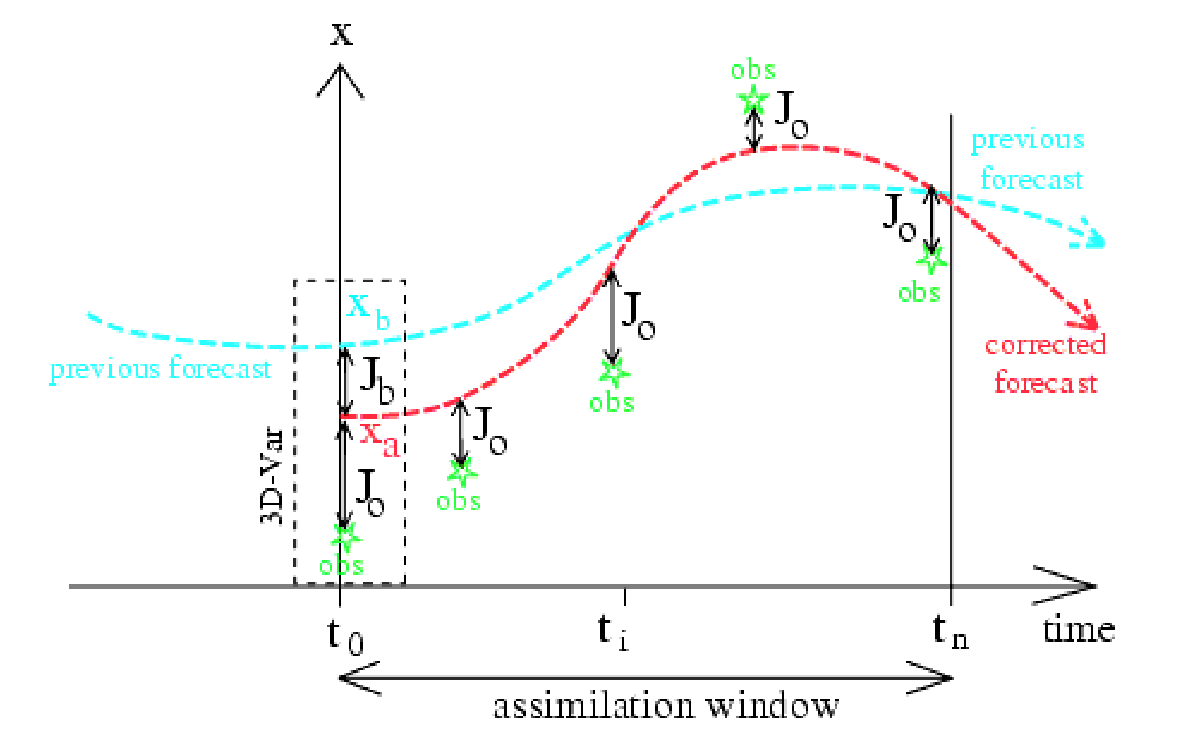
\includegraphics[scale=0.20]{4dvar_show}
\end{center}
}

\frame{
\frametitle{4D-Var versus 3D-Var\\(Adopted from ECMWF training Course)}
\begin{itemize}
	\item 4D-Var is comparing observations with background model fields at the correct time \pause
	\item 4D-Var can use observations from frequently reporting stations \pause
	\item The dynamics and physics of the forecast model in an integral part of 4D-Var, so observations are used in a meteorologically more consistent way \pause
	\item 4D-Var combines observations at different times during the 4D-Var window in a way that reduces analysis error \pause
	\item 4D-Var propagates information horizontally and vertically in a meteorologically more consistent way
\end{itemize}
}

\begin{comment}
\fst{Incremental 4D-Var formulation}{
\begin{equation*}
J=J_b+J_o
\end{equation*} \pause
Define analysis increment: $\delta\bf{x}=\bf{x}-\bf{x}_b$ \pause
\begin{equation*}
J_b=\frac{1}{2}\delta\mathbf{x}^T\mathbf{B}^{-1}\delta\mathbf{x}
\end{equation*} \pause
\begin{align*}
J_o =\frac{1}{2}\sum_{k=1}^K[(\overbrace{\mathbf{y}_k-H_kM_k\mathbf{x}_b}^{innovation}-\mathbf{H}_k\mathbf{M}_k\delta\mathbf{x})^T\mathbf{R}^{-1} \\ 
(\mathbf{y}_k-H_kM_k\mathbf{x}_b-\mathbf{H}_k\mathbf{M}_k\delta\mathbf{x})]
\end{align*} 
}

\frame{
\frametitle{Incremental 4D-Var formulation (Cont'd)}
To find the $\delta\bf{x}$ which lead the $J$ to minimal:
\begin{equation*}
\nabla_{\delta\bf{x}}{J}=0
\end{equation*} \pause
\begin{equation*}
\nabla_{\delta\bf{x}}J_b={\bf{B}^{-1}}\delta\bf{x}
\end{equation*} \pause
\begin{align*}
\nabla_{\delta\bf{x}}J_o =\sum_{k=1}^K[\underbrace{\mathbf{M}_k^T}_\text{WRF\_AD}\mathbf{H}_k^T\mathbf{R}^{-1}(\mathbf{y}_k-H_k\underbrace{M_k}_\text{WRF\_NL}\mathbf{x}_b-\mathbf{H}_k\underbrace{\mathbf{M}_k}_\text{WRF\_TL}\delta\mathbf{x})]
\end{align*} \pause
$M_k$ : Model integration from step 0 to step k. \\ \pause
$\mathbf{M}_k$ : tangent linear model and ${\mathbf{M}_k}^T$ : adjoint model are needed
}
\end{comment}

\fst{Weak constraint with digital filter}{
\begin{tabular}{l p{2in}}
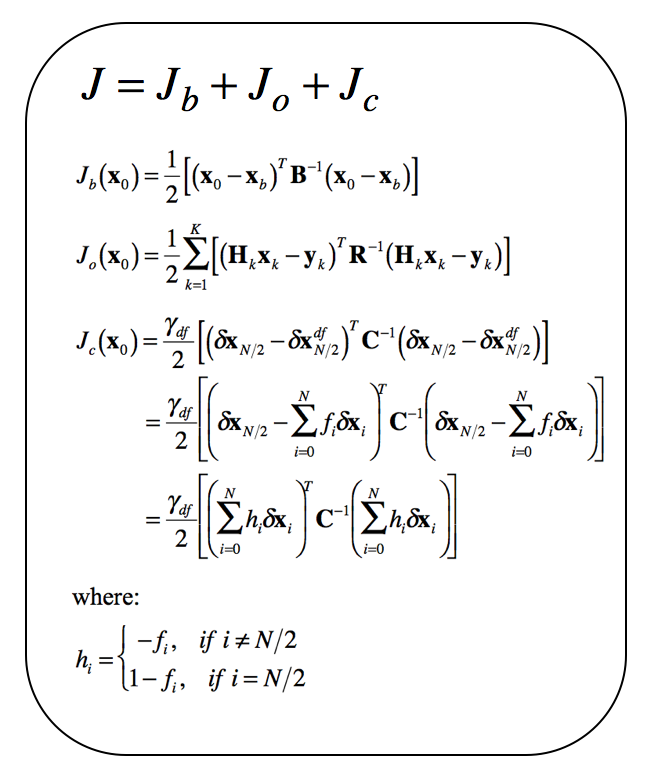
\includegraphics[scale=0.25]{jcdf_formular} \pause & 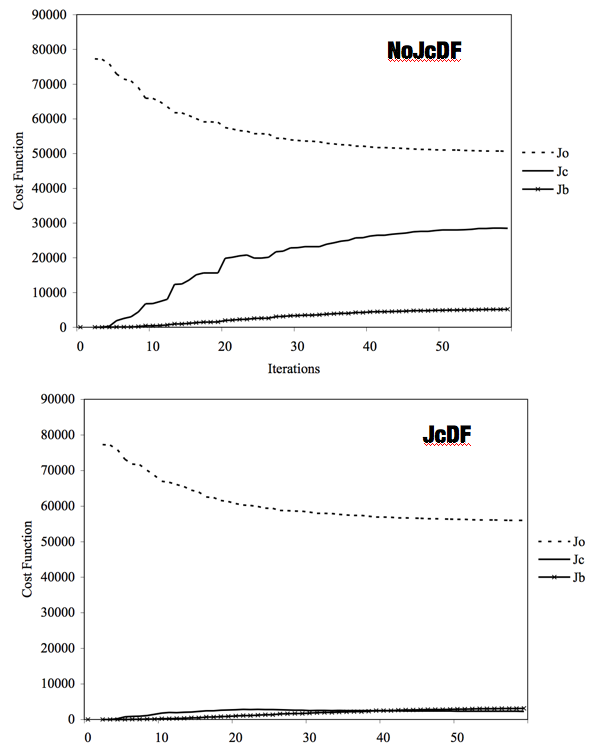
\includegraphics[scale=0.25]{jcdf}
\end{tabular}
}

\frame{
\frametitle{Weak constraint with digital filter \\(domain averaged surface pressure variation) }
\begin{center}
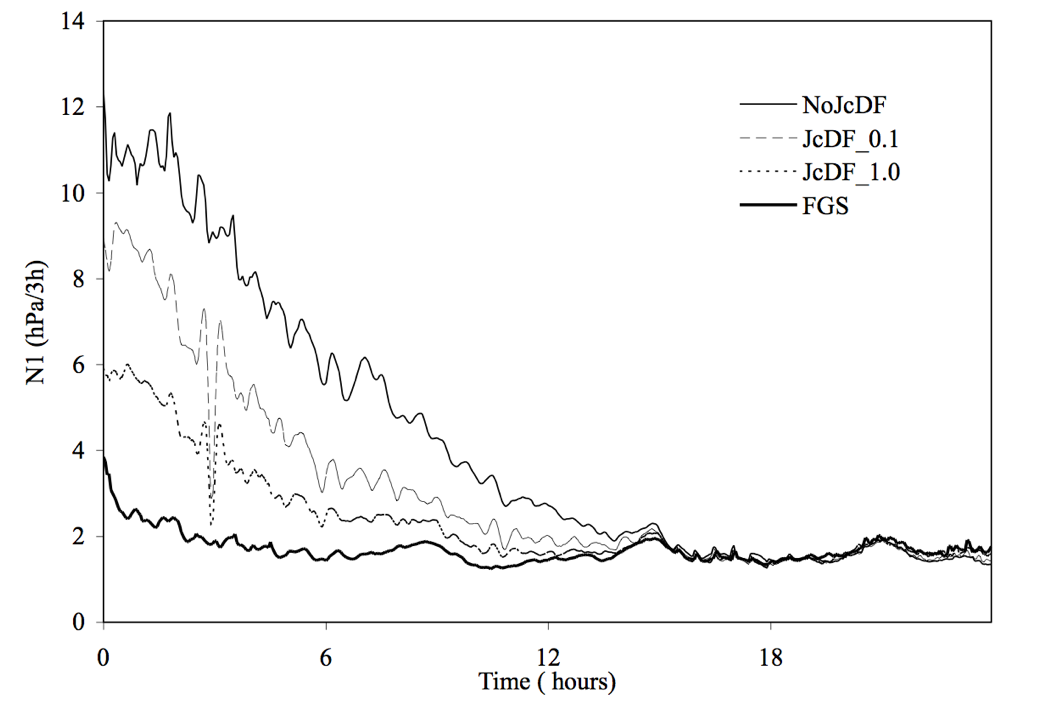
\includegraphics[scale=0.25]{jcdf_ps}
\end{center}
}

\fst{Consider lateral boundary condition as control variable}{
\begin{equation*}
J=J_b+J_o+J_c+\color{red}J_{lbc}
\end{equation*}
\begin{eqnarray*}
J_{lbc} & = & \frac{1}{2}(\mathbf{x}(t_k)-\mathbf{x}_b(t_k))^T\mathbf{B}^{-1}(\mathbf{x}(t_k)-\mathbf{x}_b(t_k))\\
& = & \frac{1}{2}\delta\mathbf{x}(t_k)^T\mathbf{B}^{-1}\delta\mathbf{x}({t_k})
\end{eqnarray*}
$J_{lbc}$ is the $J_b$ at the end of the assimilation window \\
lateral boundary control is obtained through
\begin{eqnarray*}
\frac {\partial{\delta{\mathbf{x}}_{lbc}}} {\partial{t}}=\frac{\delta\mathbf{x}(t_k)-\delta\mathbf{x}(t_0)}{t_k-t_0}
\end{eqnarray*}
}

\frame{
\frametitle{Single observation experiment}
To investigate the impact of including boundary condition control in data assimilation, a 6h observation close to boundary is put at the downstream of the boundary inflow, we expect that the major analysis increments response at 0h should be in boundary condition and outside of domain.
}

\frame{
\begin{columns}[c]
\column{5cm}
\includemovie[
  controls,poster={boundarynolbcjcdf.pdf},
  text={\large(Click to start the movie)\hspace*{400pt}}
]{6.0cm}{7.5cm}{boundarynolbcjcdf.mpeg}
\column[c]{3.5cm}
\begin{block}{Remarks}
\tiny{Forecasted 500mb T difference \\(DA forecast - reference forecast)}
\begin{itemize}
	\item {\color{red}$\star$} is the location of obs. at the ending time (6h).
	\item \tiny{$O-B=-0.95K$}
	\item \tiny{LBC control is {\color{red}turned off}}
\end{itemize}
\end{block}
\end{columns}
}

\frame{
\begin{columns}[c]
\column{5cm}
\includemovie[
  controls,poster={boundarylbcjcdf.pdf},
  text={\large(Click to start the movie)\hspace*{400pt}}
]{6.0cm}{7.5cm}{boundarylbcjcdf.mpeg}
\column[c]{3.5cm}
\begin{block}{Remarks}
\tiny{Forecasted 500mb T difference \\(DA forecast - reference forecast)}
\begin{itemize}
	\item {\color{red}$\star$} is the location of obs. at the ending time (6h).
	\item \tiny{LBC control is {\color{red}turned on}}
\end{itemize}
\end{block}
\end{columns}
}


%%%%%%%%%%%%%%%%%%%%%%%%%
\section{WRF 4D-Var Applications}

\fst{An OSSE radar data assimilation with WRF 4D-Var}{

\begin{itemize}
	\item \small{TRUTH ----- Initial condition from TRUTH (13-h forecast initialized at 	   
                           2002061212Z from AWIPS 3-h analysis) run cutted by ndown, 	     
                           boundary condition from NCEP GFS data.} \pause
	\item \small{NODA -----  Both initial condition and boundary condition from NCEP GFS data.}\pause
	\item \small{3DVAR -----3DVAR analysis at 2002061301Z used as the initial condition, and  
                           boundary condition from NCEP GFS. Only Radar radial velocity at  
                           2002061301Z assimilated (total data points = 97,033), 3 outer loops.}\pause
	\item \small{4DVAR ----- 4DVAR analysis at 2002061301Z used as initial condition, and 
                           boundary condition from NCEP GFS. The radar radial velocity at 4  
                           times: 200206130100, 05, 10, and 15, are assimilated (total
                           data points = 384,304), 3 outer loops.}
\end{itemize}
}

\frame{
\frametitle{OSSE 3rd hour precipitation simulation}
\begin{tabular}{l r}
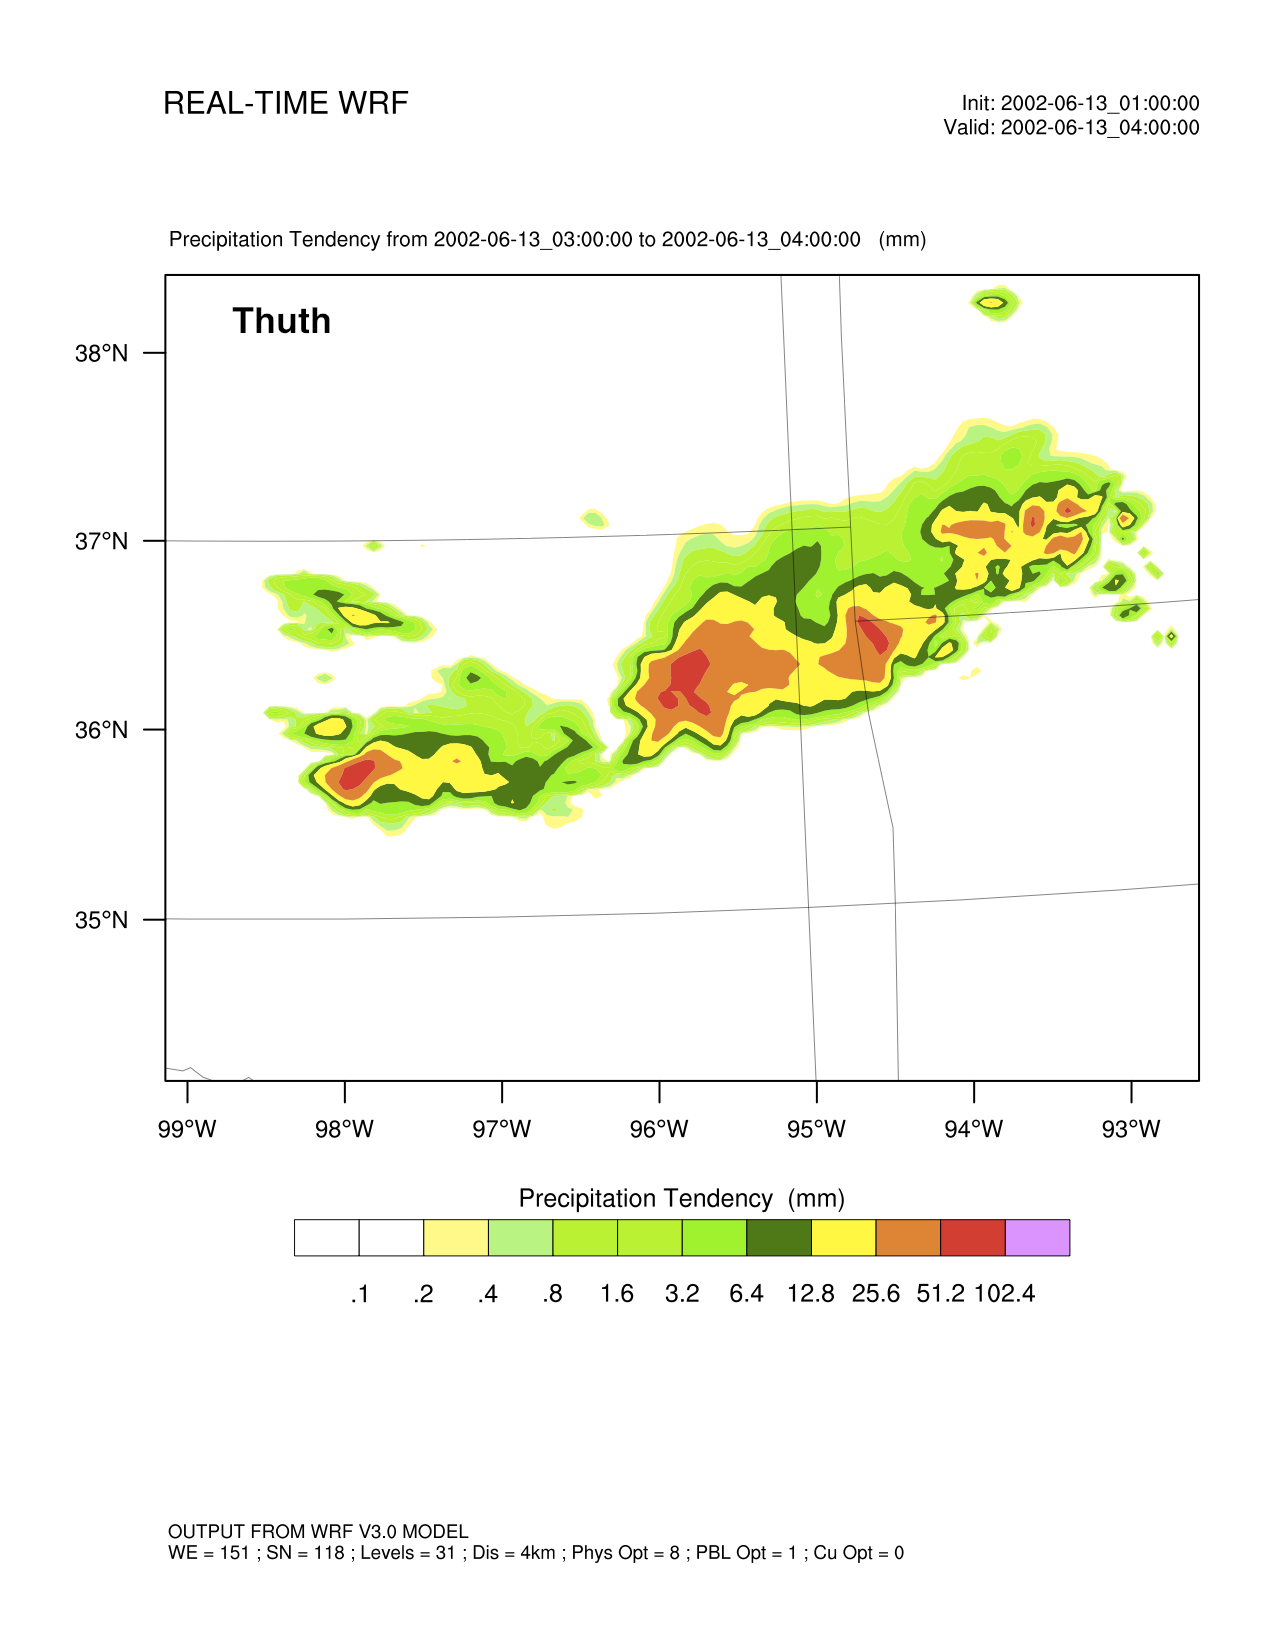
\includegraphics[scale=0.20, trim=1 240 3 100, clip]{radar_truth} & 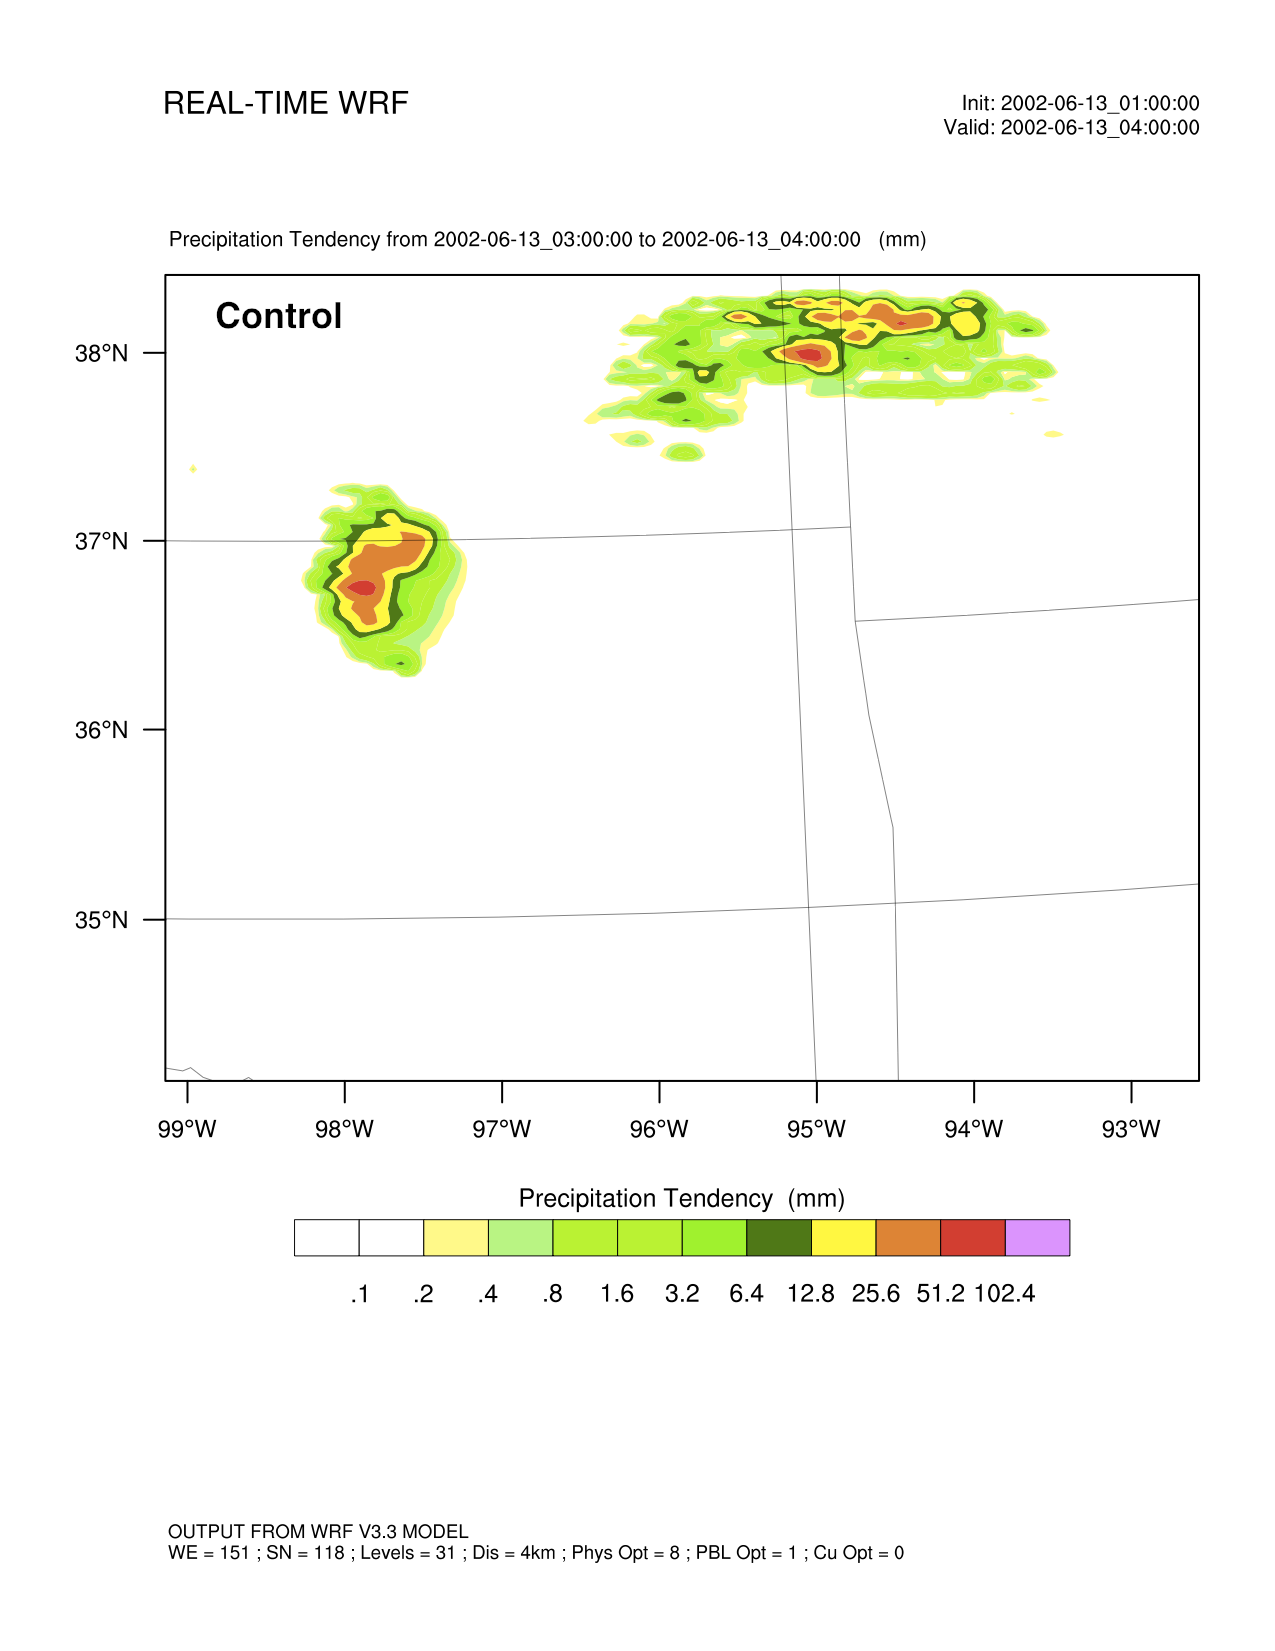
\includegraphics[scale=0.20, trim=1 240 3 100, clip]{radar_control} \\
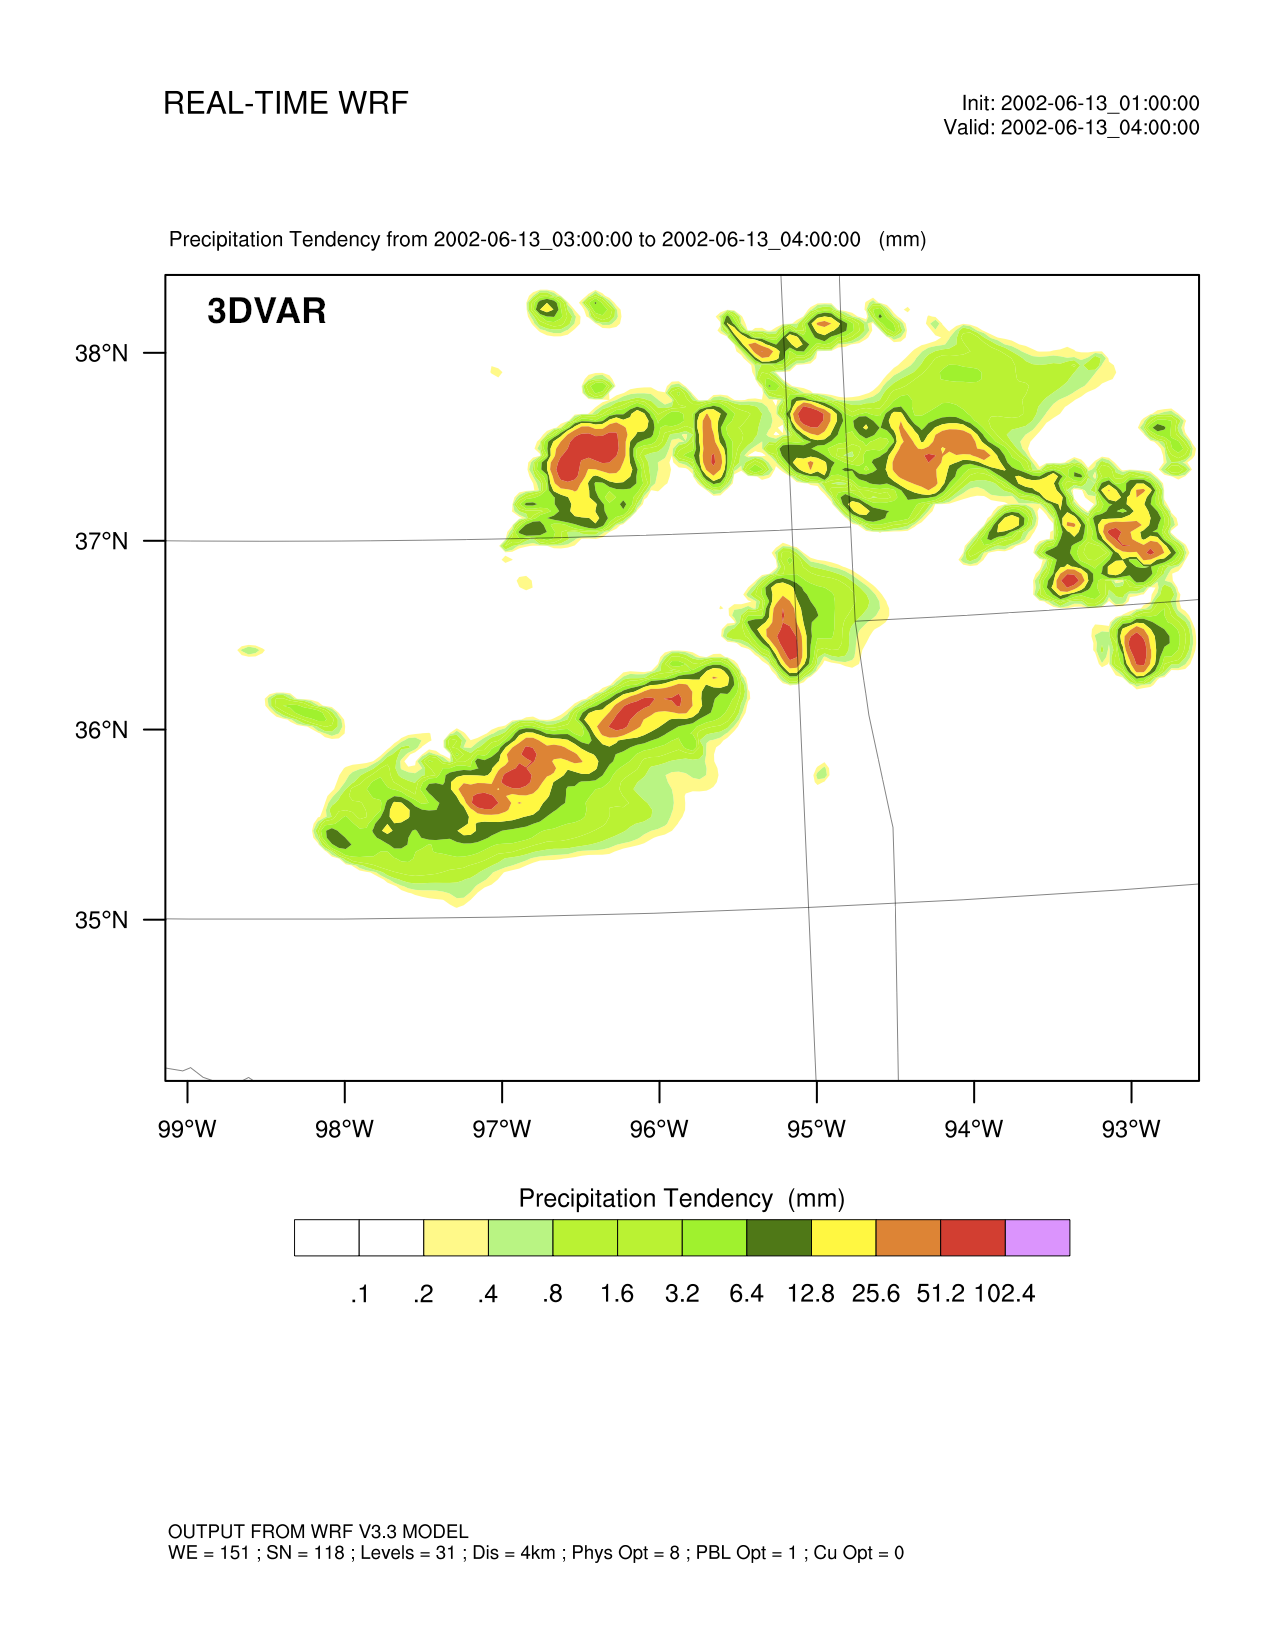
\includegraphics[scale=0.20, trim=1 160 3 130, clip]{radar_3dvar} & 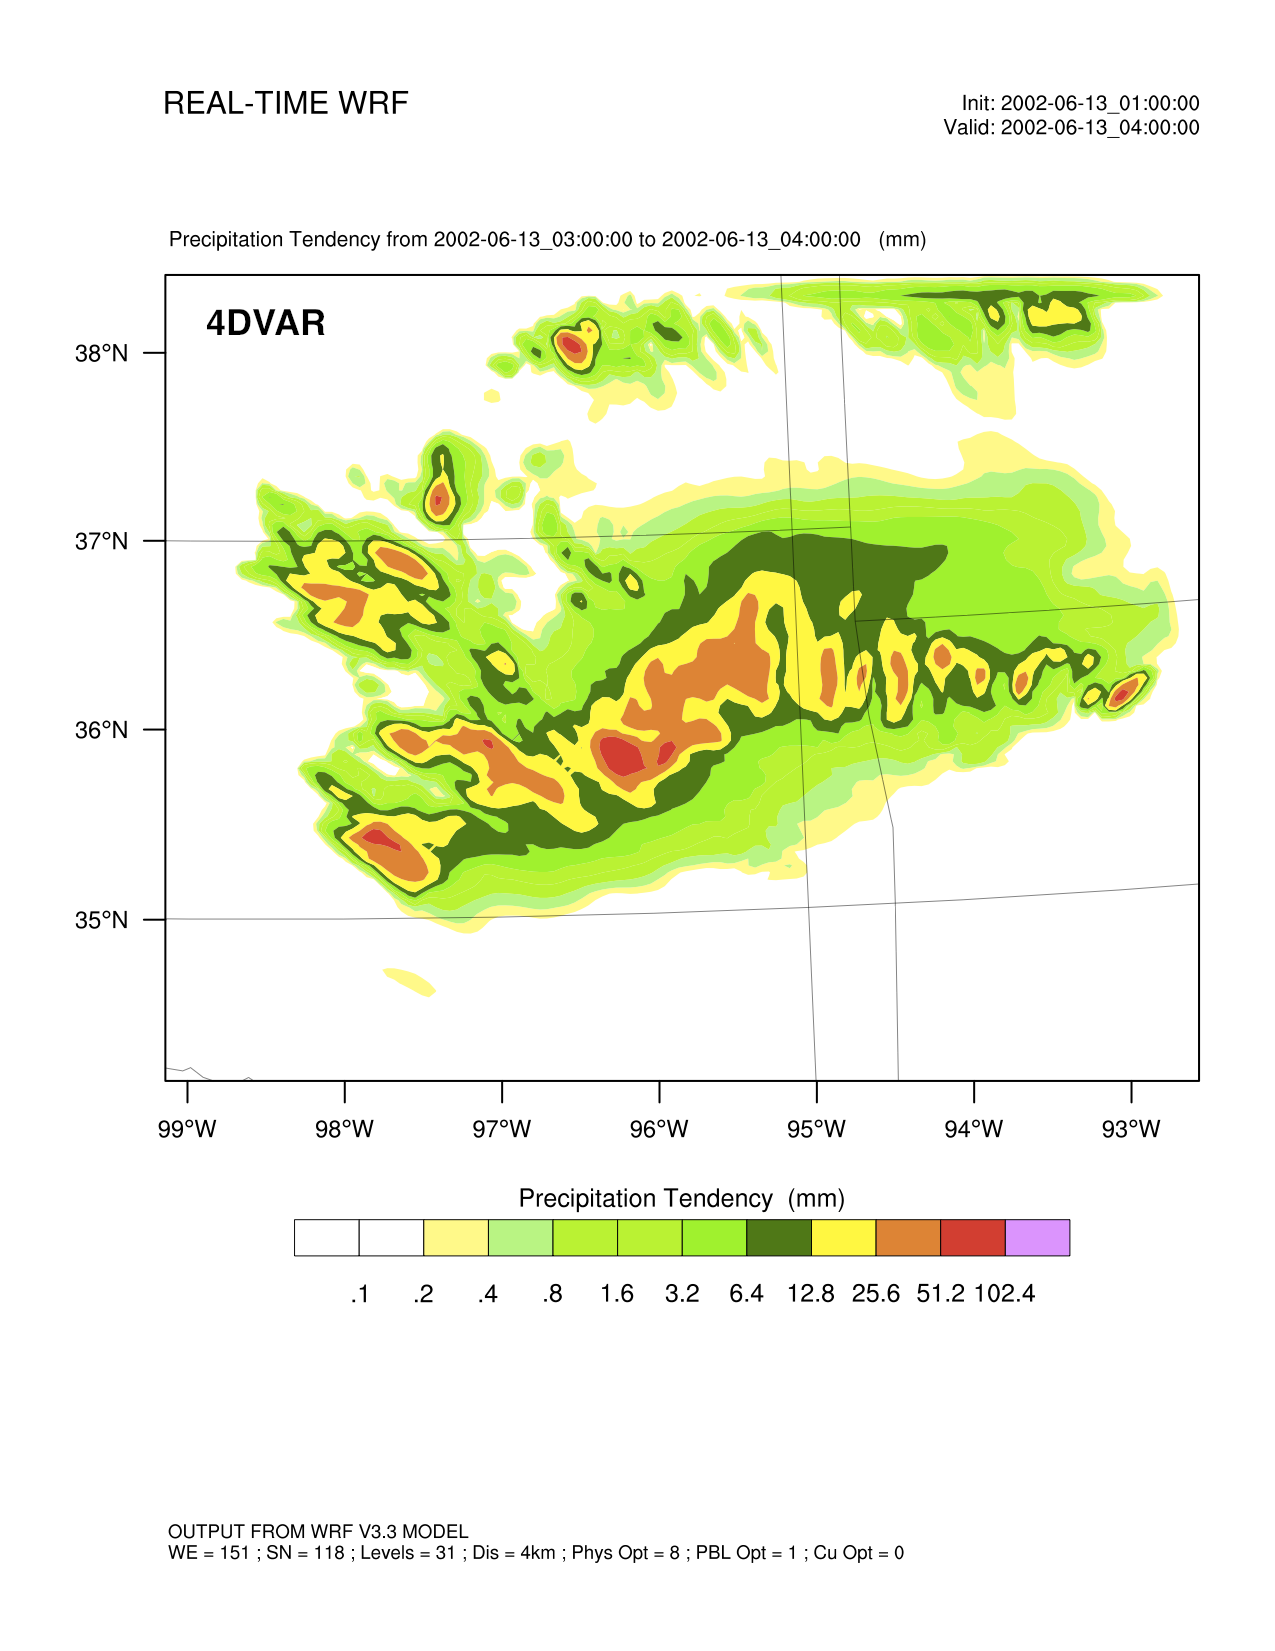
\includegraphics[scale=0.20, trim=1 160 3 130, clip]{radar_4dvar}
\end{tabular}
}

\subsection{Real case}

\frame{
\frametitle{Experiment configuration}
\begin{itemize}
	\item \tiny{Grids: 105x72x28L}
	\item Resolution: 60km
	\item Period: 2010091100-2010092600 @0Z,6Z,12Z,18Z
	\item First guess is the 12h forecast from NCEP FNL
	\item 48h forecasts from FG, 3DVAR and 4DVAR
	\item Verified against NCEP GDAS prepbufr data
\end{itemize}
\begin{center}
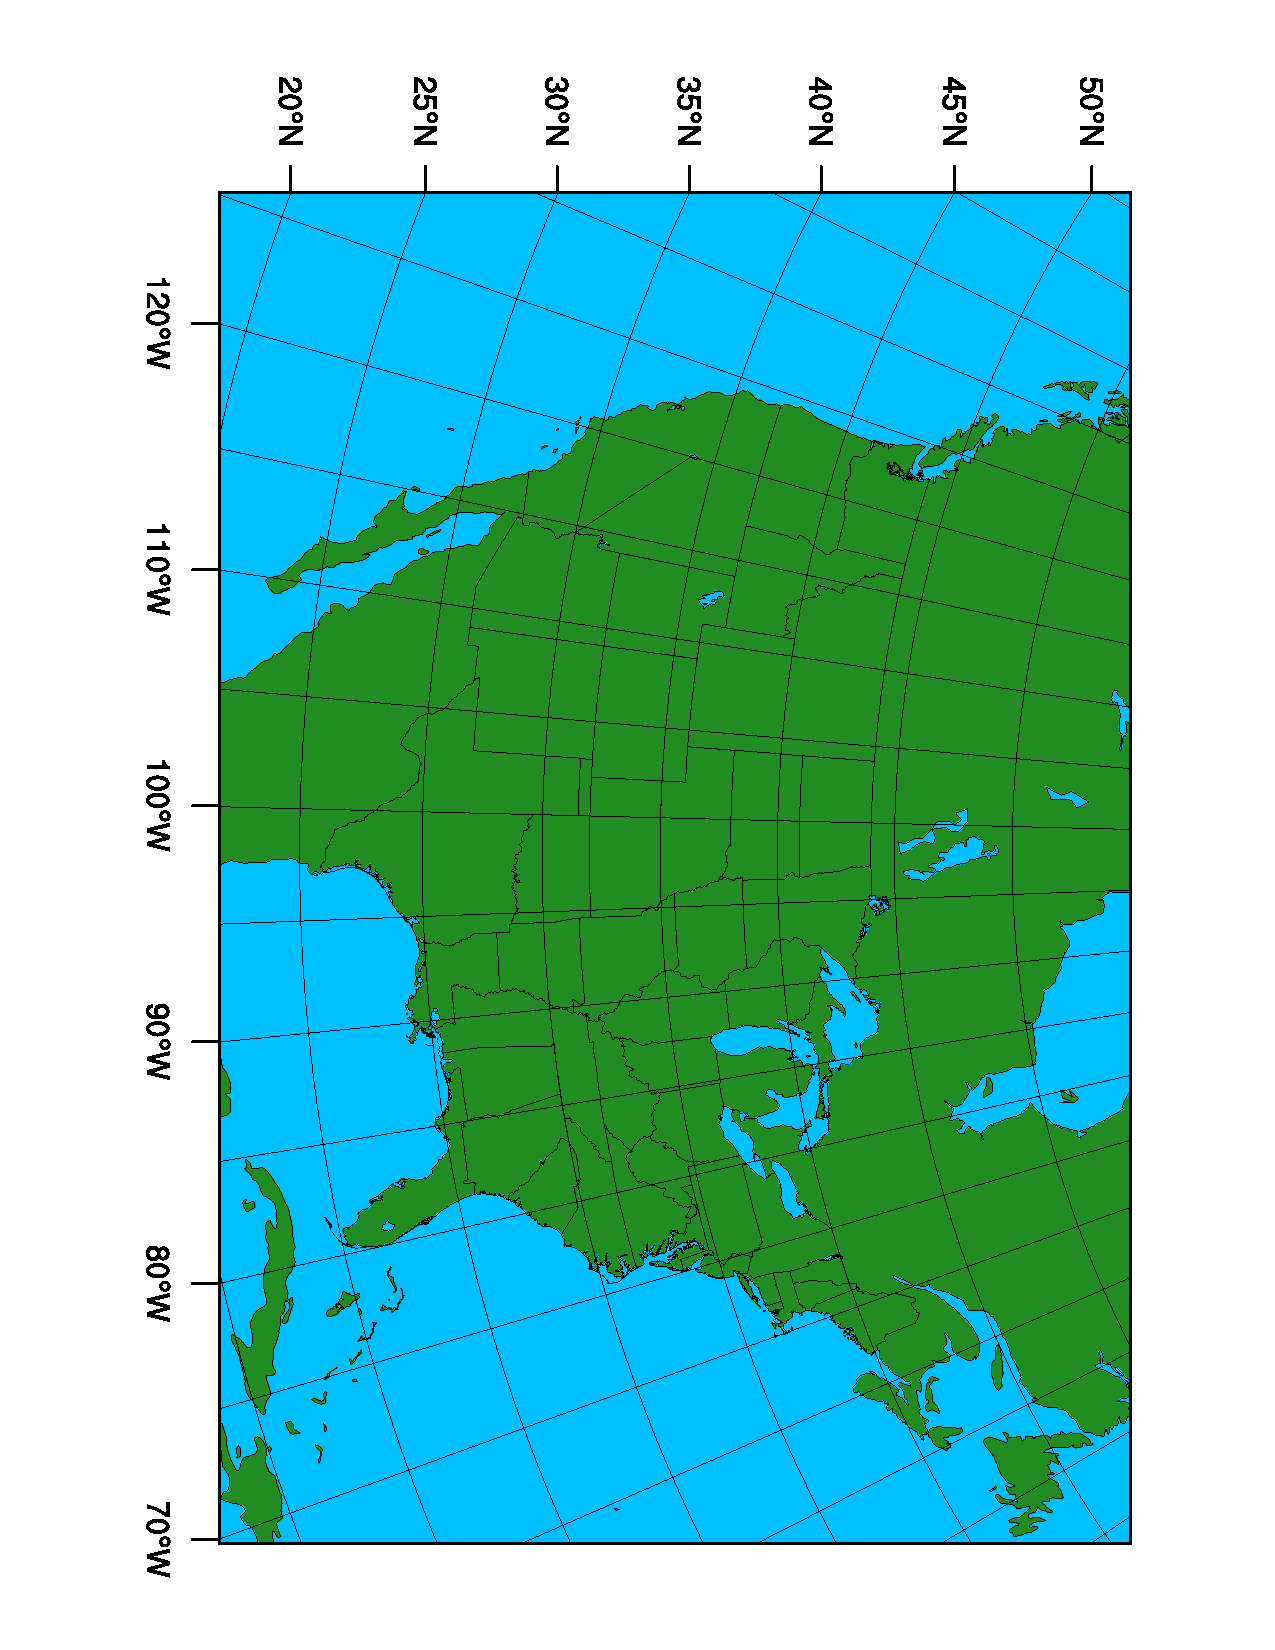
\includegraphics[scale=0.25, trim=0 0 50 0, clip, angle=90]{domain.pdf} 
\end{center}
}

\frame{
\frametitle{\small Averaged RMSE of 24H forecast verification}
\begin{center}
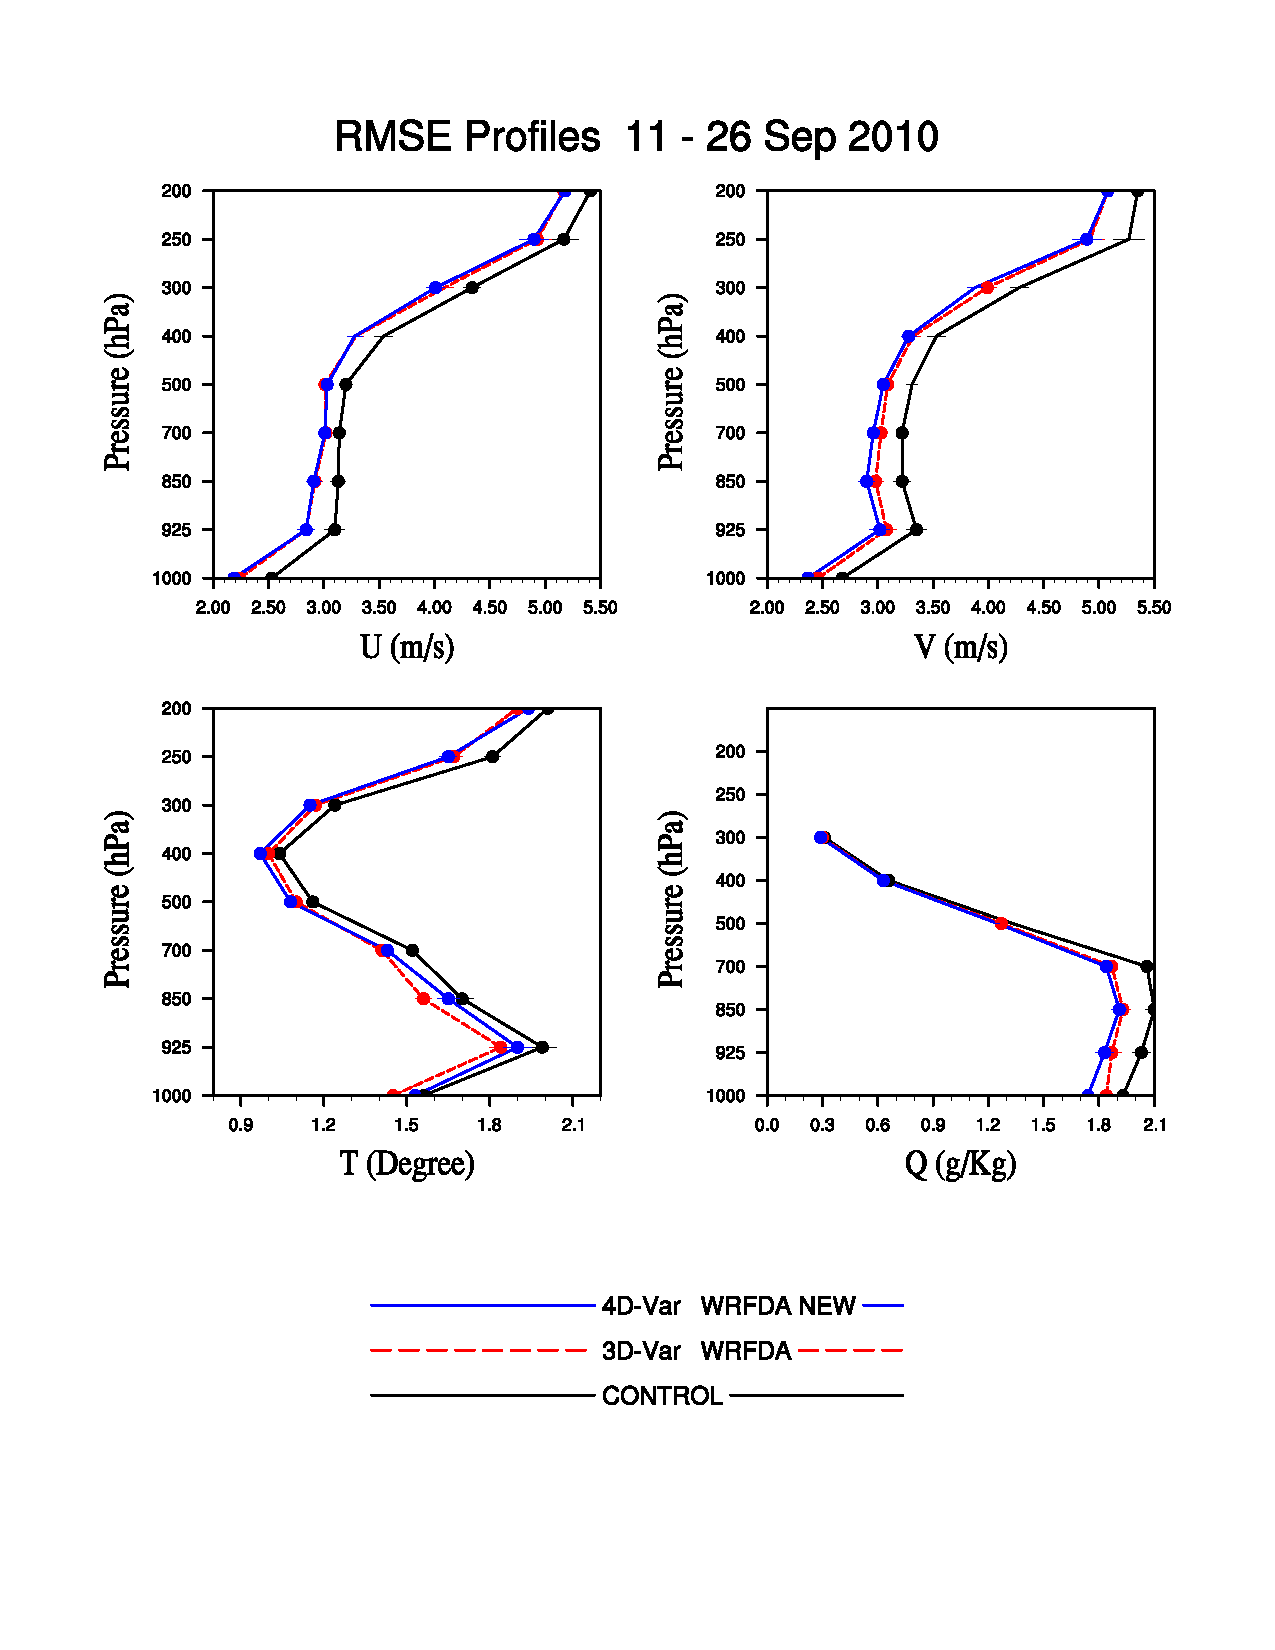
\includegraphics[scale=0.30, trim=0 100 0 55, clip]{Profile_RMSE_24H.pdf}
\end{center}
}

\frame{
\frametitle{\small Averaged RMSE of 36H forecast verification}
\begin{center}
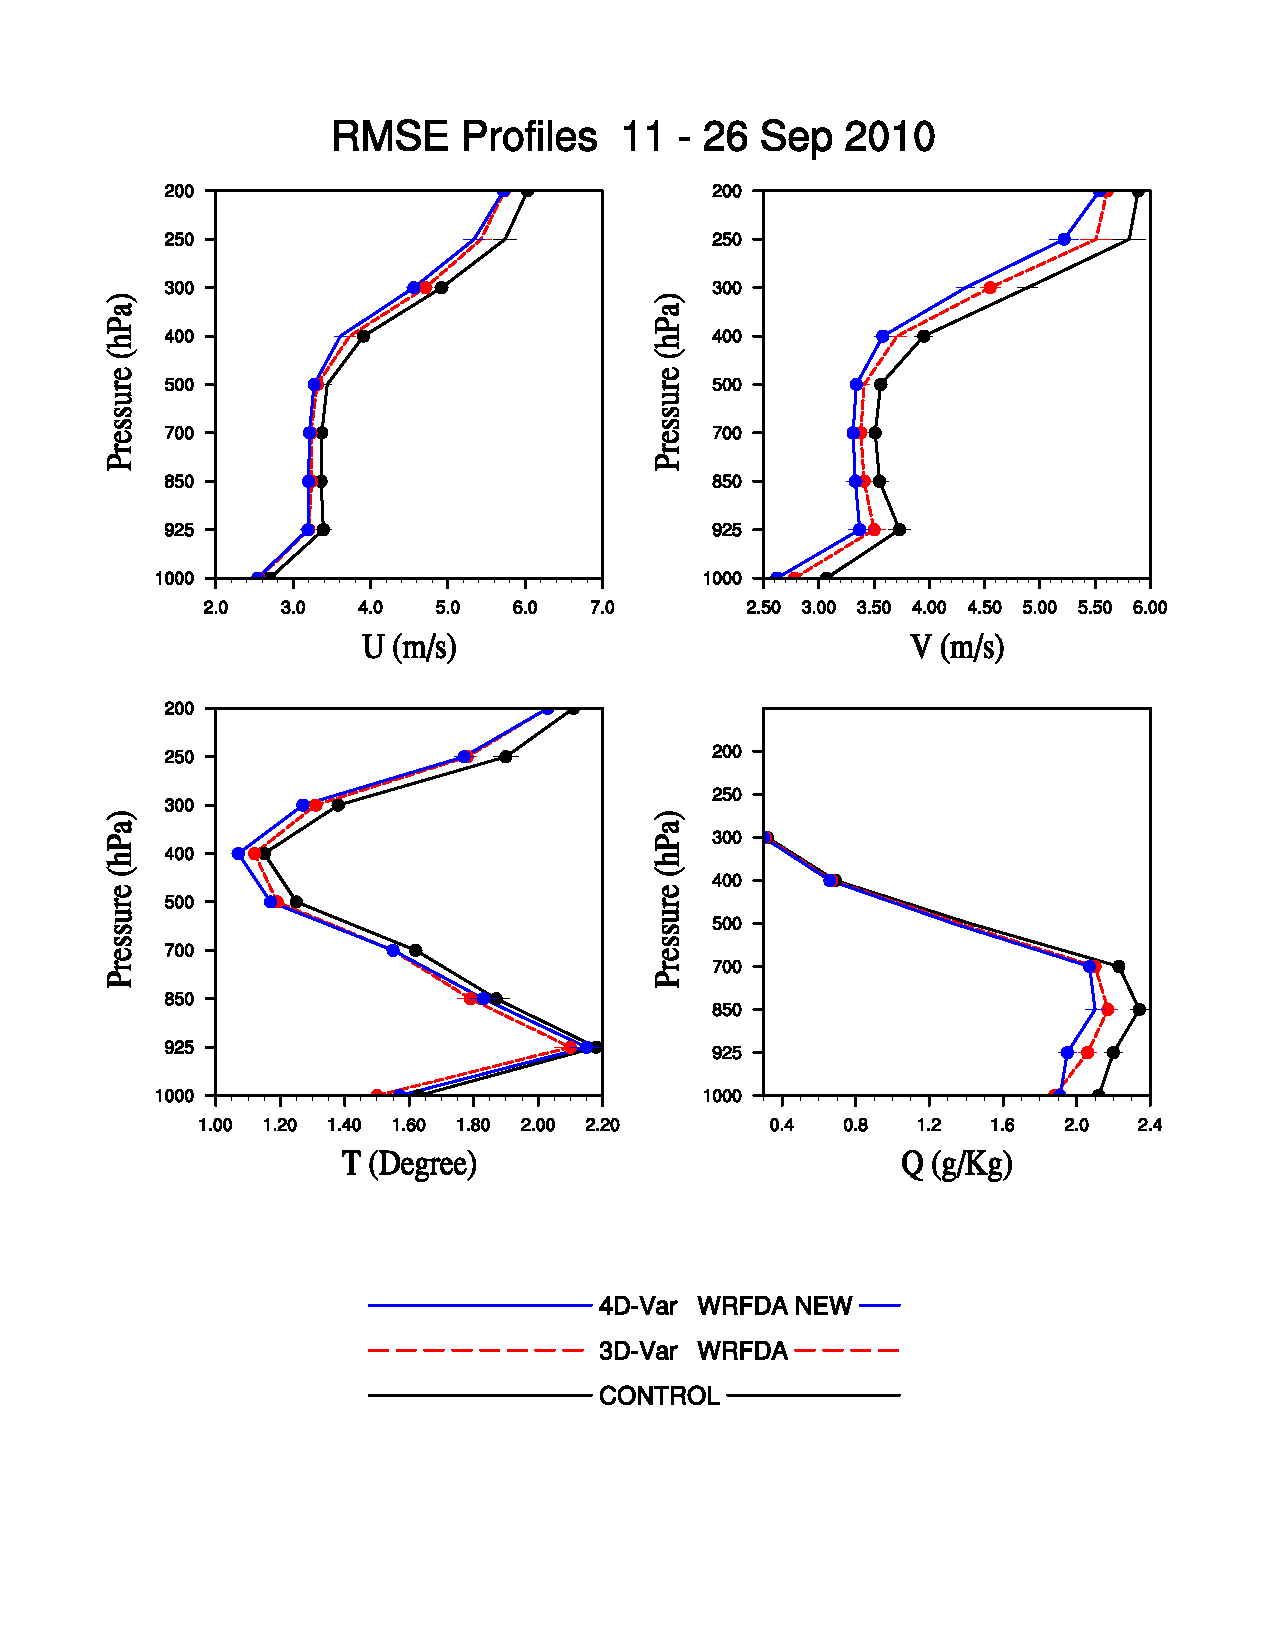
\includegraphics[scale=0.30, trim=0 100 0 55, clip]{Profile_RMSE_36H.pdf}
\end{center}
}

\frame{
\frametitle{\small Averaged RMSE of 48H forecast verification}
\begin{center}
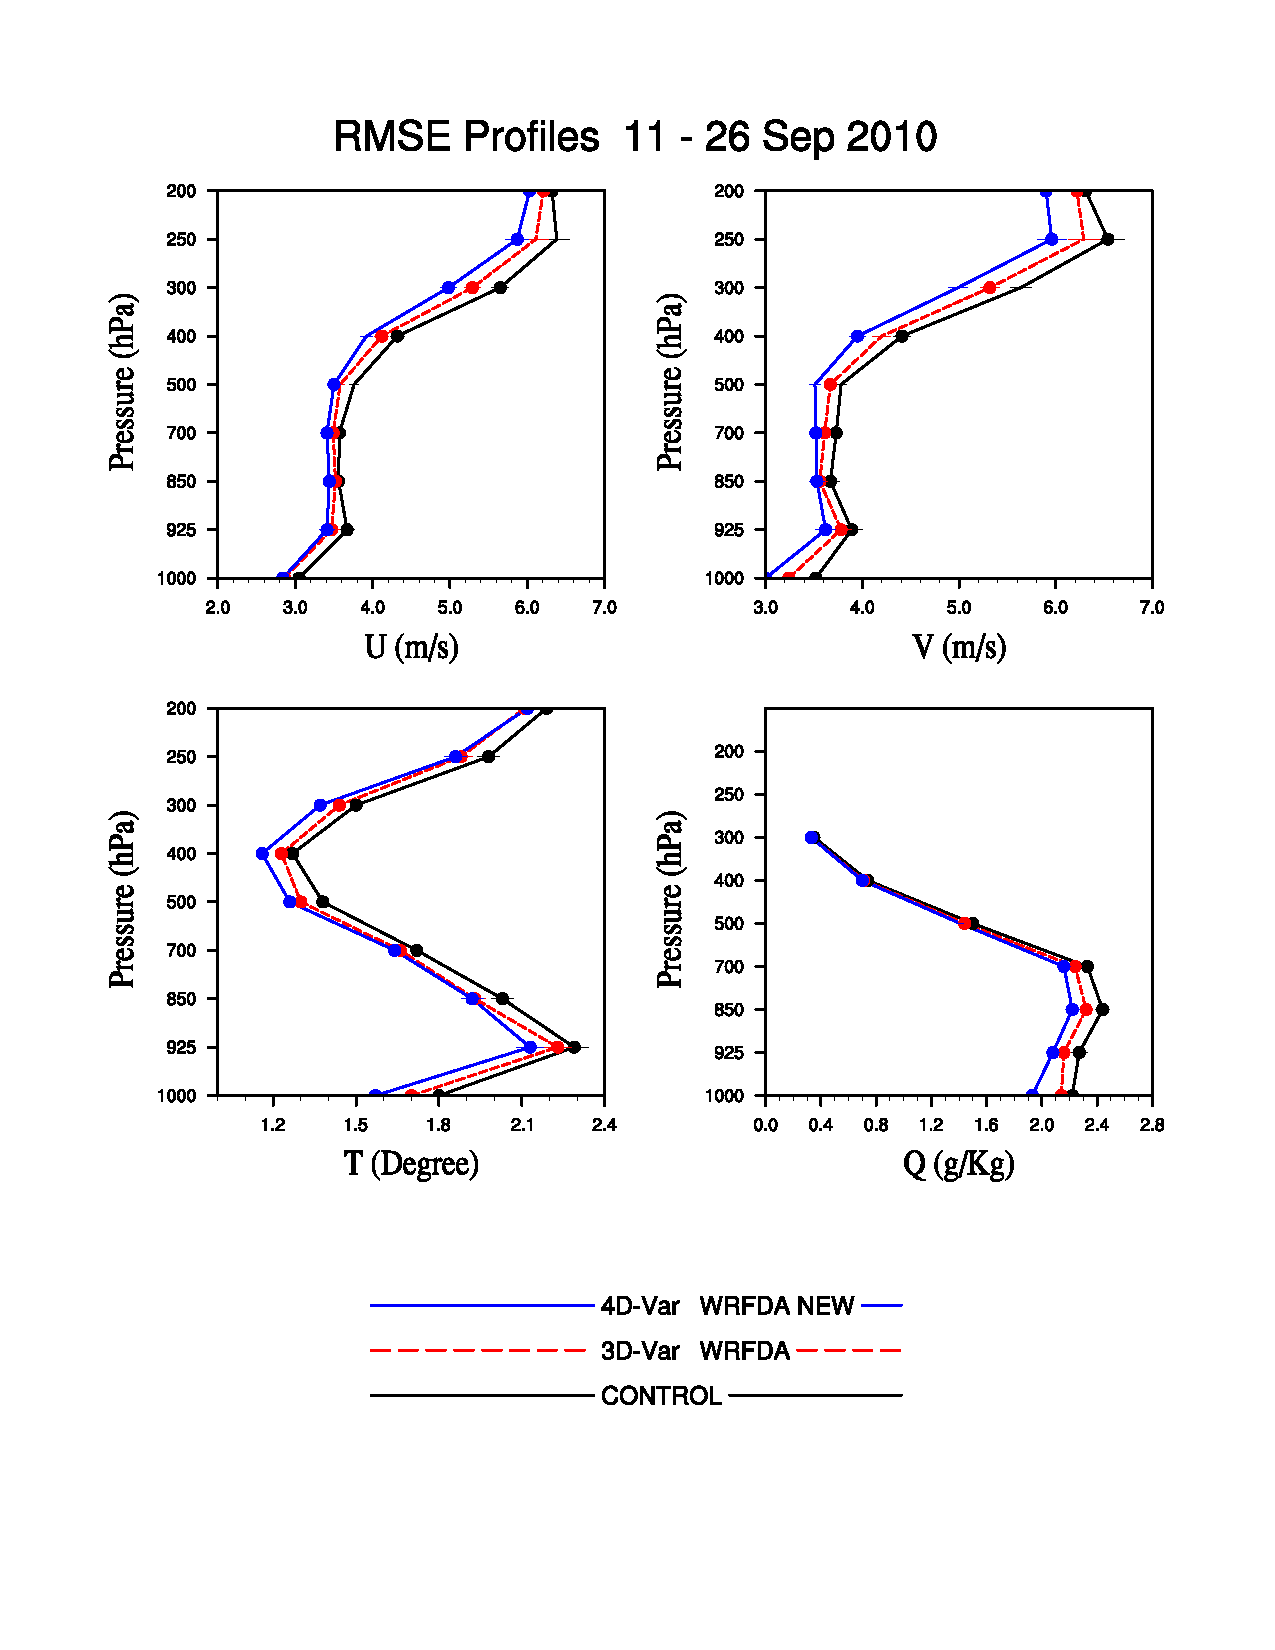
\includegraphics[scale=0.30, trim=0 100 0 55, clip]{Profile_RMSE_48H.pdf}
\end{center}
}

%%%%%%%%%%%%%%%%%%%%%%%%%%%%%%%%%
\section{WRF 4D-Var Setup}

\frame{
\frametitle{Download and setup test dataset for this tutorial}
\begin{itemize}
	\item download the WRFDAcodes from :\\
		{\tiny\url{http://www.mmm.ucar.edu/wrf/users/wrfda/download/get_source.html}}\pause
	\item download the WRFPLUSV3 codes  and the patch from :\\
		{\tiny\url{http://www.mmm.ucar.edu/wrf/users/wrfda/download/wrfplus.html}}
		{\tiny\url{http://www.mmm.ucar.edu/wrf/users/wrfda/known-prob_V3_3.html}}\pause
	\item enter into WRFDA/var/test/4dvar \pause
	\item get the test dataset from :\\
		{\tiny\url{ftp://ftp.ucar.edu/pub/mmm/xinzhang/WRF4DVar_V3.3_Tutorial/2008020521}}\pause
	\item $ln$ $-fs$ $wrfinput\_d01$ $fg$ \pause
	\item $ln$ $-fs$ $../../build/da\_wrfvar.exe$ $.$
	\item $ln$ $-fs$ $../../run/be.dat.cv3$ $be.dat$
\end{itemize}
}
\fst{Installation}{
\begin{itemize}
   \item Install WRFPLUS V3.3
   	\begin{itemize}
   	 	\item $./configure$  $(-d)$  $wrfplus$
   	     	\item $./compile$  $em\_real$
		\item $wrf.exe$ should be generated under $main$ directory.
   	 \end{itemize}\pause
    \item for csh, tcsh : {\small{$setenv$  $WRFPLUS\_DIR$  $path\_of\_wrfplusv3$}}
    \item for bash, ksh : {\small{$export$  $WRFPLUS\_DIR=path\_of\_wrfplusv3$}}\pause
    \item Install WRFDA V3.3
        \begin{itemize}
    	\item $./configure$  $(-d)$  $4dvar$
	\item $./compile$  $all\_wrfvar$
	\item $da\_wrfvar.exe$ should be generated under $var{\slash}build$ directory.
    \end{itemize}
\end{itemize}
}

\frame{
\frametitle{Tips for compilation}
\begin{itemize}
   	\item Speed up the compilation with parallel make ---gnu make:  \\
		{\small{$setenv$  $J$  $"-j$ $6"$}} \pause
   	\item {\small{$setenv$  $BUFR$  $1$}} to assimilate prepbufr observation. \pause
	\item {\small{$setenv$  $CRTM$  $1$}} to assimilate radiance bufr data with CRTM.
\end{itemize}
}

\frame{
\frametitle{Portability}
We have tested the WRF 4D-Var V3.3 on following systems:
\begin{itemize}
   	\item IBM with XLF compiler V12.1 \pause
   	\item Linux with PGI compiler V8.0-4 64-bit \pause
	\item Linux with INTEL compiler V11.1 \pause
	\item Mac with PGI compiler V10.3-0 64-bit \pause
	\item Mac with GFORTRAN compiler V4.4.0  \pause
	\item Mac with G95 compiler V4.0.3 (please download the patch on WRFDA home page)
\end{itemize}
}

\frame{
\frametitle{Common problems in compilation}
\begin{itemize}
   	\item To use gfortran (default 32-bit) on Mac snow leopard system, "-m64" need to be manually appended after "SFC" in $configure.wrf$ \pause
	\item Enough memory is needed to compile some subroutines in WRFPLUS with default optimization level (-O3). Manually reduce the compilation optimization level for some subroutines when system can not allocate enough memory to perform compilation with higher level optimization. \pause
	\item On some platforms, some compilers might not be able to compile WRF with real\_size=8. Usually, upgrading the compiler is the easiest way to solve this problem.
\end{itemize}
}

\fst{Test for tangent linear model and adjoint model}{
\begin{itemize}
   	\item After WRFPLUS compilation, It is a good practice to run tangent linear model test and adjoint model test with you own case IC and BC.  \pause
	\item Under $WRFPLUSV3/test/em\_real$ directory, a test case are setup to let users test the tangent linear model and adjoint model. \pause
	\item In $namelist.input$, turn on $check\_TL$ and/or $check\_AD$ in $\&perturbation$ to run tangent linear check or adjoint check.
\end{itemize}
}

\frame[containsverbatim]{
\frametitle{Test for tangent linear model}
Taylor formula:
\begin{equation*}
\lim_{\alpha \to 0}\frac{M(x+\alpha\delta\mathbf{x})-M(x)}{M^{'}({\alpha\delta\mathbf{x}})}=1
\end{equation*}
\begin{block}{check results}
{\tiny{
\begin{verbatim}
 =============== Tangent Linear check ===================
 check==== U === V === W == PH === T == MU == MOIST =====
 check     T     T     T     T     T     T     T
alpha_m=.1000E+00  coef=   0.98250076417818E+00  val_n= 0.3628649E+11  val_l= 0.3693279E+11
alpha_m=.1000E-01  coef=   0.99781045126907E+00  val_n= 0.3685192E+09  val_l= 0.3693279E+09
alpha_m=.1000E-02  coef=   0.99949153238165E+00  val_n= 0.3691401E+07  val_l= 0.3693279E+07
alpha_m=.1000E-03  coef=   0.10002560538015E+01  val_n= 0.3694225E+05  val_l= 0.3693279E+05
alpha_m=.1000E-04  coef=   0.99981685944643E+00  val_n= 0.3692603E+03  val_l= 0.3693279E+03
alpha_m=.1000E-05  coef=   0.10000972073298E+01  val_n= 0.3693638E+01  val_l= 0.3693279E+01
alpha_m=.1000E-06  coef=   0.99996624597337E+00  val_n= 0.3693154E-01  val_l= 0.3693279E-01
alpha_m=.1000E-07  coef=   0.99999992233716E+00  val_n= 0.3693279E-03  val_l= 0.3693279E-03
alpha_m=.1000E-08  coef=   0.10000017668820E+01  val_n= 0.3693285E-05  val_l= 0.3693279E-05
alpha_m=.1000E-09  coef=   0.10000050602279E+01  val_n= 0.3693298E-07  val_l= 0.3693279E-07
alpha_m=.1000E-10  coef=   0.10000451984913E+01  val_n= 0.3693446E-09  val_l= 0.3693279E-09
\end{verbatim}
}}
\end{block}
}

\frame[containsverbatim]{
\frametitle{Test for adjoint model}
adjoint identity:
\begin{equation*}
\forall\mathbf{x}, \forall\mathbf{y} : \langle{M^{'}.\mathbf{x},\mathbf{y}}\rangle =  \langle{\mathbf{x},\mathbf{M^{*}}.\mathbf{y}}\rangle
\end{equation*}
\begin{block}{check results}
{\tiny{
\begin{verbatim}
 ad_check: VAL_TL:    0.41466174569087E+11
 ad_check: VAL_AD:    0.41466174569088E+11
\end{verbatim}
}}
\end{block}
\begin{itemize}
   	\item Although the tangent linear model might be imperfect.
	\item The adjoint test must be perfect. otherwise, there are bugs in the adjoint model.
\end{itemize}
}

\frame{
\frametitle{Answers to frequently asked questions regarding to WRFPLUS}
\begin{itemize}
	\item WRFPLUS only works with regional ARW core, not for NMM core or global WRF. \pause 
   	\item WRFPLUS only works with single domain, not for nested domains.  \pause
	\item WRFPLUS can not work with Adaptive Time Stepping options. \pause
	\item WRFPLUS only has three simplified physics processes: surface drag (bl\_pbl\_physics=9); large scale condensate (mp\_physics=98);a simplified cumulus scheme (cu\_physics=98)
\end{itemize}
}

\fst{WRF 4D-Var observation preparation}{
\begin{itemize}
   	\item Conventional observation --- LITTLE\_R format \\
	         {\tiny\url{http://www.mmm.ucar.edu/wrf/users/wrfda/Tutorials/2010\_Aug/docs/WRFDA\_obsproc.pdf}} \pause
   	\item {\color{red} OR} Conventional observation --- prepbufr format
		\begin{itemize}
			\item {\tiny{near real-time data : \url{ftp://ftp.ncep.noaa.gov/pub/data/nccf/com/gfs/prod}}}
			\item {\tiny{history archives : \url{http://dss.ucar.edu/dataset/ds337.0}}}
		\end{itemize} \pause
	        	\item Satellite radiance bufr data
		\begin{itemize}
			\item {\tiny{near real-time data : \url{ftp://ftp.ncep.noaa.gov/pub/data/nccf/com/gfs/prod}}}
			\item {\tiny{history archives : \url{http://dss.ucar.edu/dataset/ds735.0}}}
		\end{itemize} \pause
	\item Ascii formated Radar data\\
		 {\tiny\url{http://www.mmm.ucar.edu/wrf/users/wrfda/Tutorials/2010\_Aug/docs/WRFDA\_radar.pdf}}
\end{itemize}
}

\frame{
\frametitle{Tips for using prepbufr and bufr data on non-IBM platforms}
 On non-IBM platforms,the prepbufr and bufr formats observation downloaded from NCEP ftp server or NCAR achives should be converted. This conversion was conducted using the C code ssrc.c located in the $utils$ directory of the GSI distribution. \\
 ~\\
More detail information and GSI codes download, please refer to \\ {\tiny\url{http://www.dtcenter.org/com-GSI/users/support/faqs/index.php}}

\begin{itemize}
	\item How to compile ssrc.c: \\
		{\tiny{pgcc -o ssrc.exe ssrc.c}}
	\item How to convert : \\
		{\tiny{ssrc.exe $<$ prepbufr.gdas.2008020600.wo40 $>$ ob.bufr \\
		ssrc.exe $<$ gdas.1bamua.t00z.20080206.bufr $>$ amusa.bufr}}
\end{itemize}
}
%%%%%%%%%%%%%%%%%%%%%%%%%%%%%%%%%
\section{WRF 4D-Var Run}


\fst{Important namelist variables for 4D-Var run}{
\begin{itemize}
	\item $\&wrfvar1$
	\begin{itemize}
		\item $var4d$: logical, if run 4D-Var
		\item $var4d\_lbc$ : logical, if include lateral boundary condition control in 4D-Var
		\item $var4d\_bin$: integer, seconds, length of sub-window to group observations in 4D-Var
	\end{itemize} \pause
	\item $\&perturbation$
		\begin{itemize}
		\item $trajectory\_io$: logical, do not change, testing purpose
		\item $enable\_identity$ : logical, if run TL/AD model with identity model, testing purpose
		\item $jcdfi\_use$: logical, if turn on the digital filter as a weak constraint.
		\item $jcdfi\_diag$: integer, 0/1, $J_c$ term diagnostics
		\item $jcdfi\_penalty$: real, weight to jcdf term
	\end{itemize}
\end{itemize}
}

\frame{
\frametitle{Important namelist variables for 4D-Var run, cont'd}
\begin{itemize}
	\item $\&physics$
	\begin{itemize}
		\item all physics options must be consistent with which used in wrfinput or fg
	\end{itemize} \pause
	\item $\&wrfvar18,21,22$
	\begin{itemize}
		\item $analysis\_date$ is the start time of the assimilation window
		\item $time\_window\_min$ is the start time of the assimilation window
		\item $time\_window\_max$ is the end time of the assimilation window
	\end{itemize} \pause
	\item $\&time\_control$
	\begin{itemize}
		\item $run\_xxxxs$ must be consistent with the length of the assimilation window
		\item $start\_xxxx$ must be consistent with the start time of the assimilation window
		\item $end\_xxxx$ must be consistent with the end time of the assimilation window
	\end{itemize}
\end{itemize}
}

\subsection{How to run WRF 4D-Var}

\frame[containsverbatim]{
\frametitle{Adjoint check before 4D-Var run}
It is always a good practice to run adjoint check before the product run.
How:   
\begin{itemize}
\item 
\tiny
\begin{verbatim}
	&wrfvar10
		test_transforms=true,
\end{verbatim}
	\item run \begin{verbatim}da_wrfvar.exe\end{verbatim}
\end{itemize}

\begin{block}{Check results}
{\tiny{
\begin{verbatim}
...
 wrf: back from adjoint integrate
 d01 2008-02-05_21:00:00 read nonlinear xtraj time stamp:2008-02-05_21:00:00
 Single Domain < y, y     > =   2.15435506772433E+06
 Single Domain < x, x_adj > =   2.15435506772431E+06

 Whole Domain < y, y     > =   2.15435506772433E+06
 Whole Domain < x, x_adj > =   2.15435506772431E+06

da_check_xtoy_adjoint: Test Finished:

 *** WRF-Var check completed successfully ***
\end{verbatim}
}}
\end{block}
}

\frame{
\frametitle{Symmetric 4D-Var window}
\begin{center}
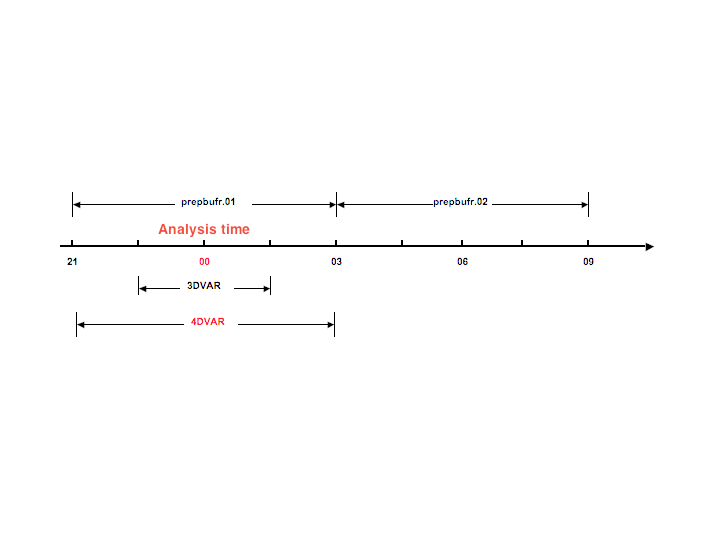
\includegraphics[scale=0.40,trim=1 120 1 120, clip]{obs_usage0}
\end{center}
\begin{itemize}
	\item IC \& BC for 3D-Var is valid for 00Z
	\item IC \& BC for 4D-Var is valid for 21Z
\end{itemize}
}

\frame{
\frametitle{Comparison of obs. usage on 2008020600}
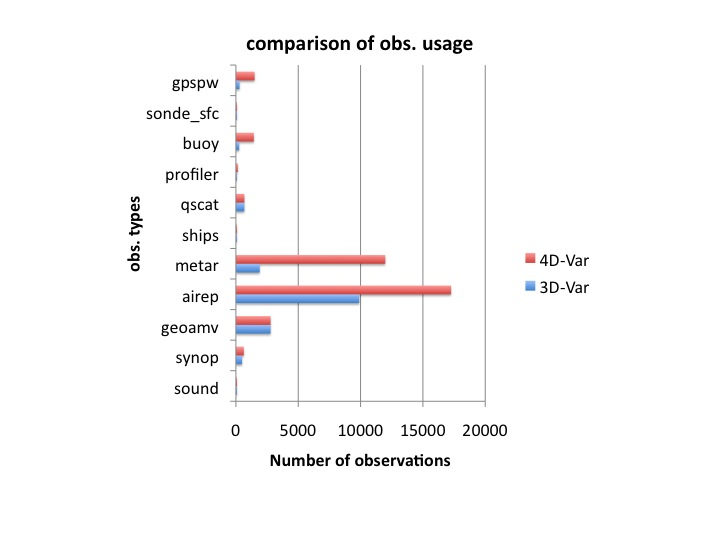
\includegraphics[scale=0.45, trim=0 40 30 60, clip]{obs_number}
}

\frame{
\frametitle{Minimization comparison}
\begin{center}
\begin{tabular}{c c}
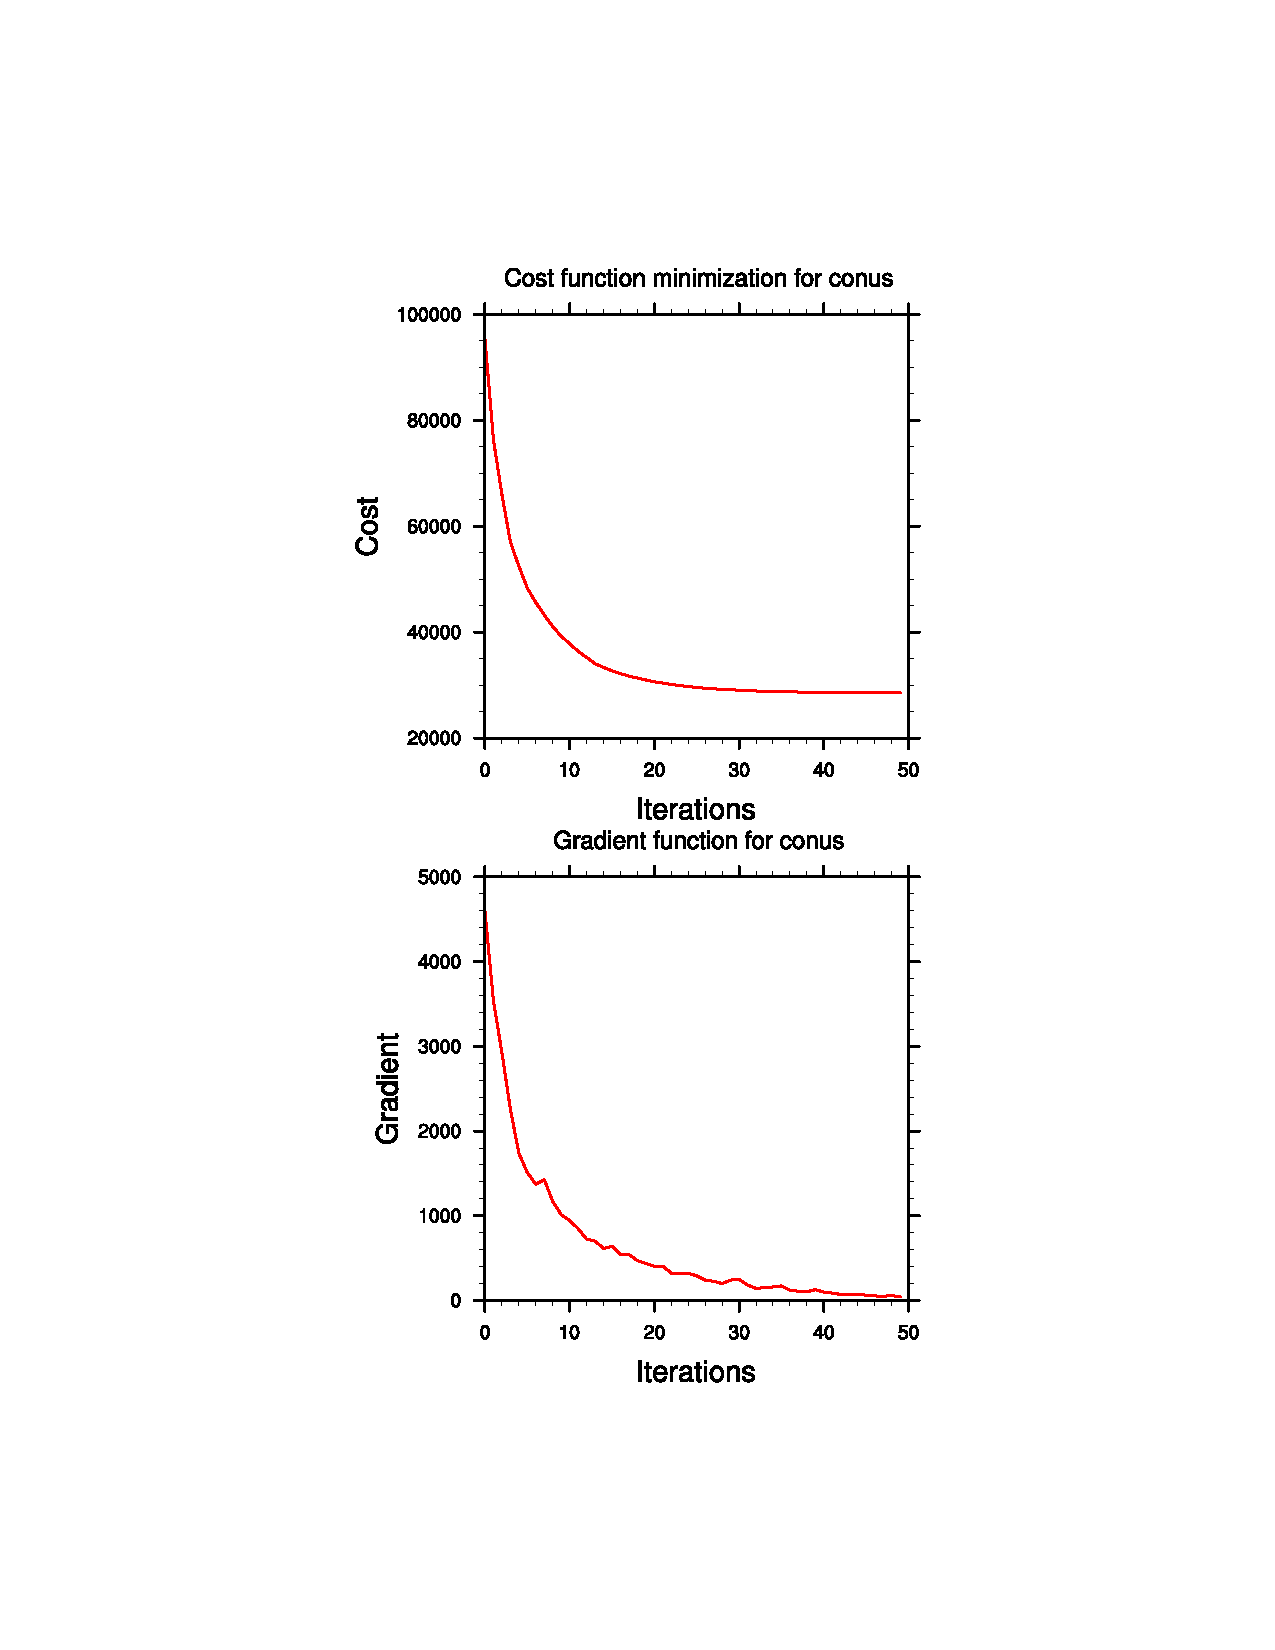
\includegraphics[scale=0.30, trim=150 120 150 120, clip]{cost_grad_3dvar} & 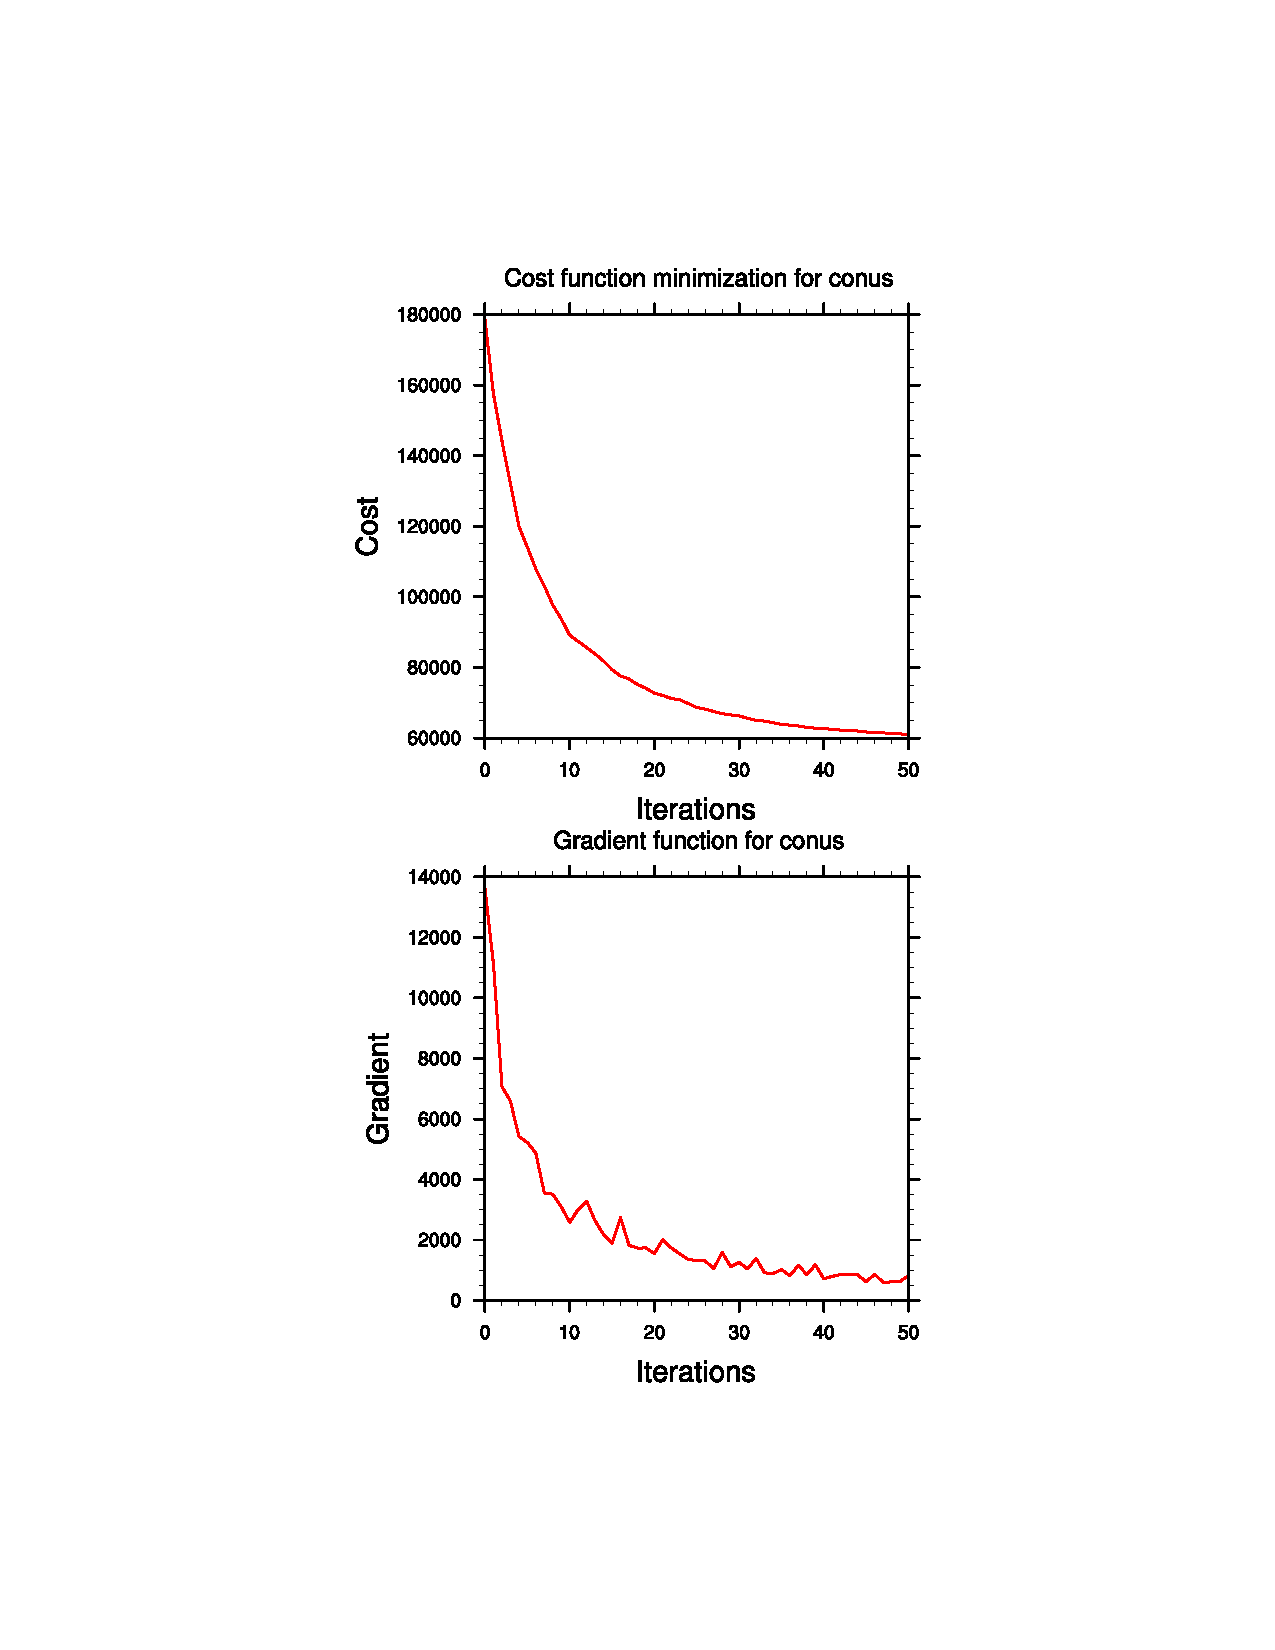
\includegraphics[scale=0.30, trim=150 120 150 120, clip]{cost_grad_4dvar} \\
{\tiny{3D-Var}} & {\tiny{4D-Var}}
\end{tabular}
\end{center}
}

\frame{
\frametitle{Sample analysis increments valid on 2008020600}
\begin{center}
\begin{tabular}{c c}
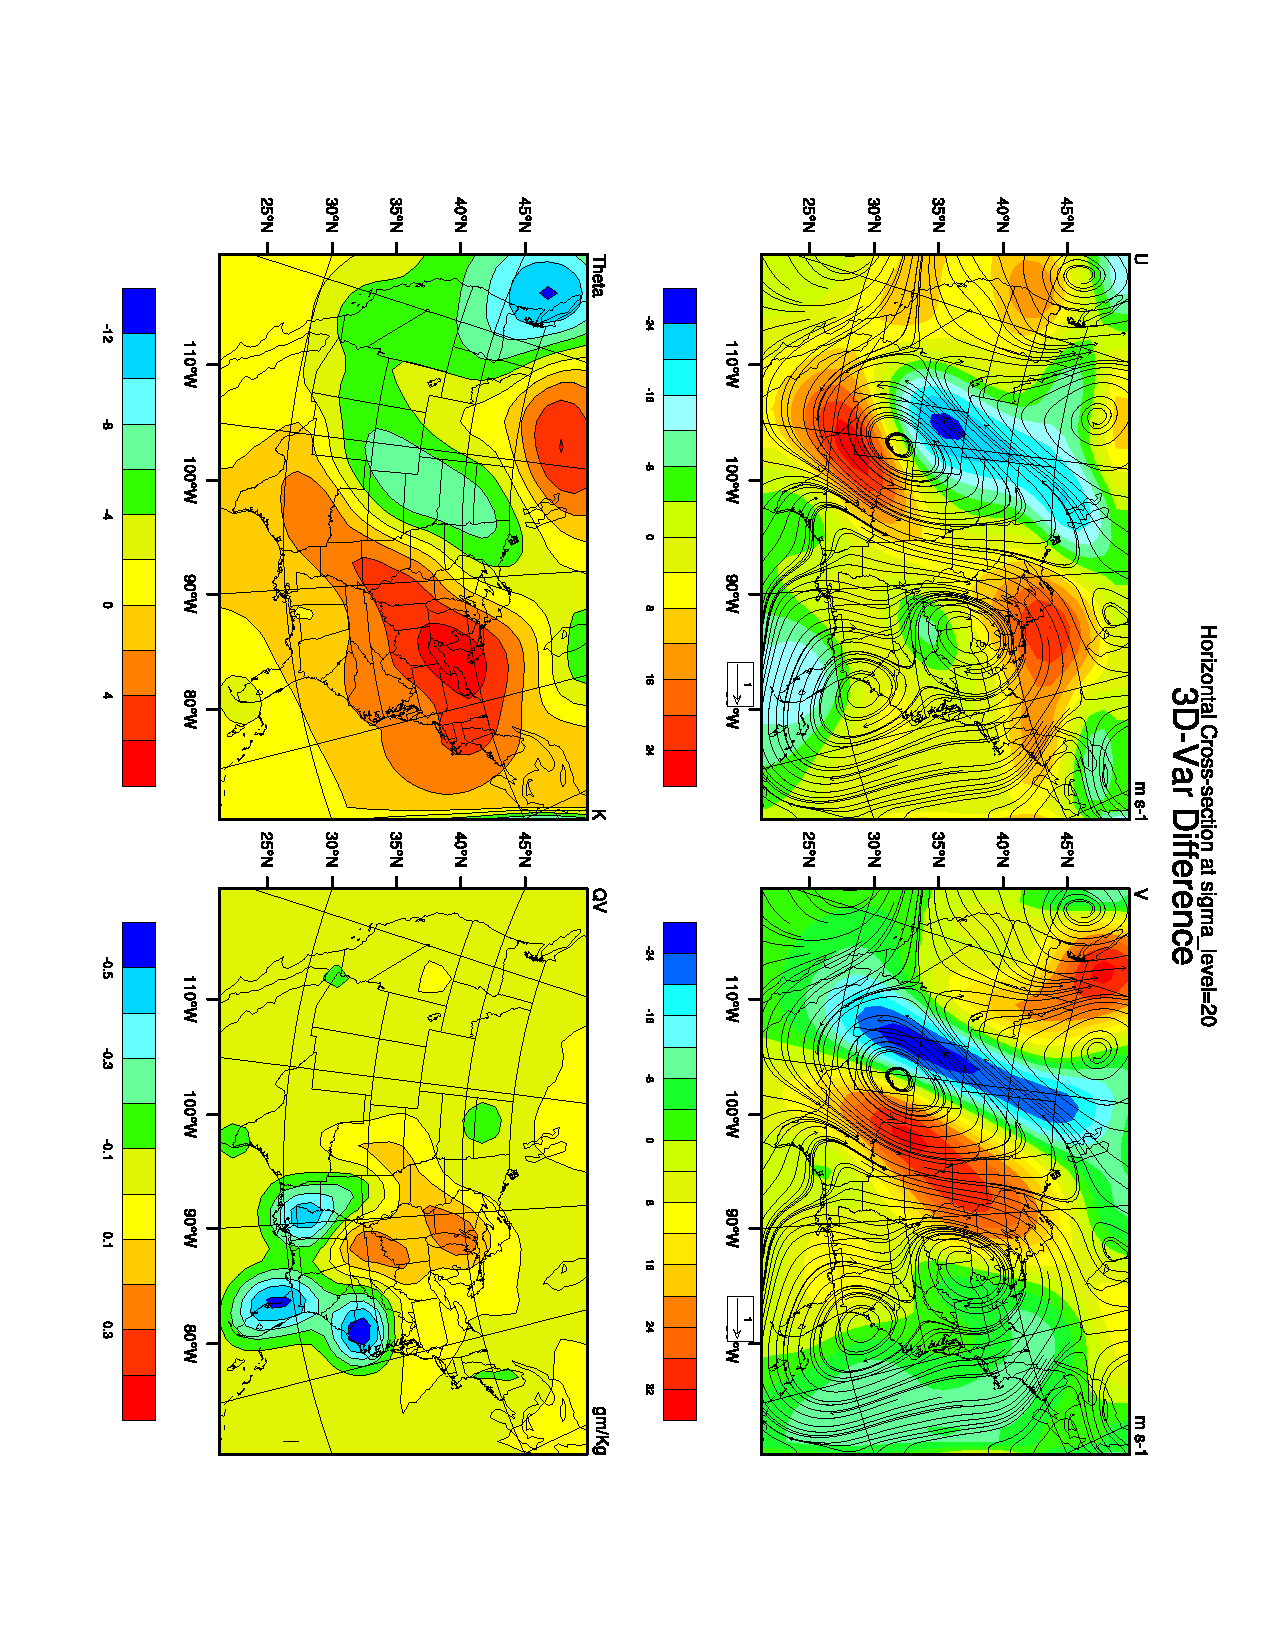
\includegraphics[scale=0.25, angle=90, trim=1 80 3 80, clip]{diff_sigma_20_3dvar} & 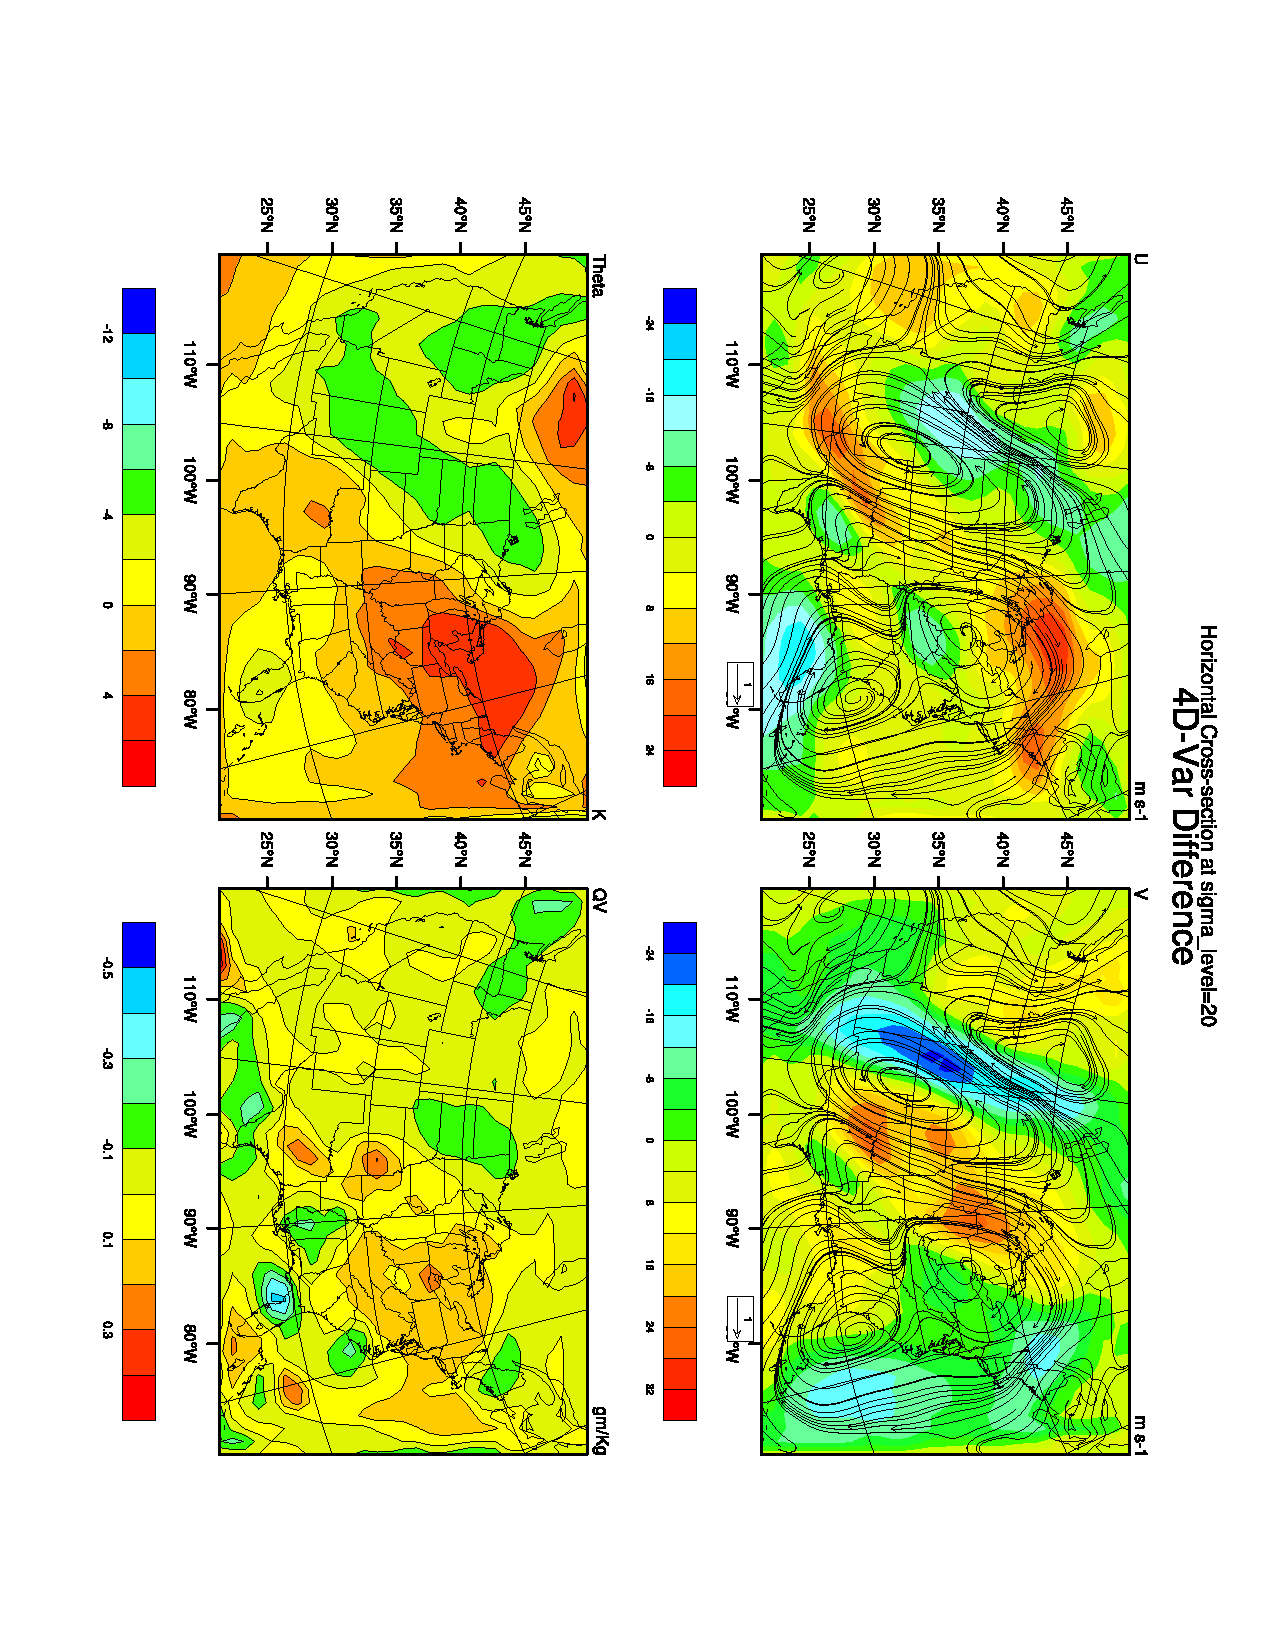
\includegraphics[scale=0.25, angle=90, trim=1 80 3 80, clip]{diff_sigma_20_4dvar}
\end{tabular}
\end{center}
}

\subsection{Assimilate satellite radiance data}

\frame[containsverbatim]{
\frametitle{Assimilate satellite radiance data}
refer to WRFDA Users' guide Chapter 6: \\
\tiny{\url{http://www.mmm.ucar.edu/wrf/users/wrfda/Docs/user_guide_V3.3/users_guide_chap6.htm#_Radiance_Data_Assimilations}} \\
~\\
Modify namelist.input for radiance data :
\tiny
\begin{verbatim}
&wrfvar4
	use_amsuaobs=true,
	use_amsubobs=true,
&wrfvar14
	rtminit_nsensor=6,
	rtminit_platform=1,1,1,1,1,1,
	rtminit_satid=15,16,18,15,16,17,
	rtminit_sensor=3,3,3,4,4,4,
	thinning_mesh=120.0,120.0,120.0,120.0,120.0,120.0,
	thinning=true,
	qc_rad=true,
	rtm_option=2,
	use_varbc=true,
	use_crtm_kmatrix=true,
\end{verbatim}
}

\frame{
\frametitle{Additional links for radiance assimilation}
\begin{itemize}
	\item link/copy amsua data as $amsua.bufr$
	\item link/copy amsub data as $amsub.bufr$
	\item $link$ $-fs$ $WRFDA/var/run/radiance\_info$ $radiance\_info$
	\item $link$ $-fs$ $WRFDA/var/run/crtm\_coeffs$ $crtm\_coeffs$
\end{itemize}
}

\frame{
\frametitle{One-side 4D-Var window}
\begin{center}
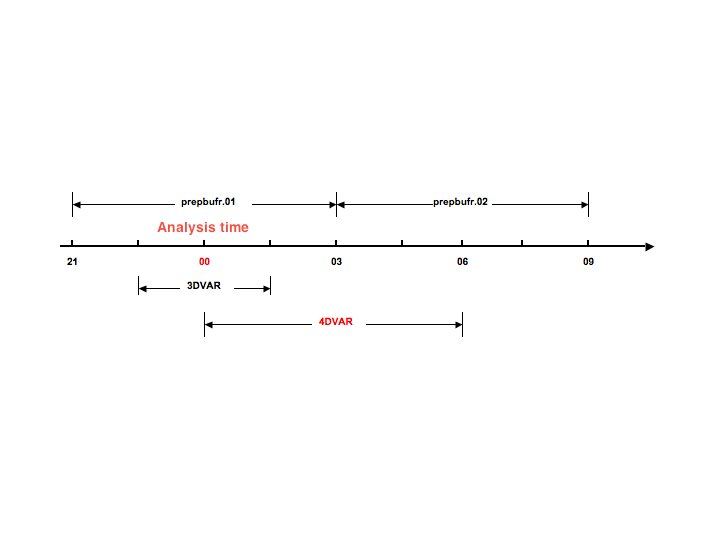
\includegraphics[scale=0.30,trim=1 120 1 120, clip]{obs_usage}
\end{center}
\pause
\begin{itemize}
	\item link/copy prepbufr data at \alert{00}Z as $ob\alert{01}.bufr$
	\item link/copy prepbufr data at \alert{06}Z as $ob\alert{02}.bufr$\pause
	\item link/copy amsua data at \alert{00}Z as $amsua\alert{01}.bufr$
	\item link/copy amsua data at \alert{06}Z as $amsua\alert{02}.bufr$
	\item \dots
\end{itemize}
}

\subsection{Common problems in WRF 4D-Var run}

\frame[containsverbatim]{
\frametitle{Common problems in WRF 4D-Var run}
	
	{\tiny{
	\begin{block}{Error message}
	\begin{verbatim}
 **************BUFR ARCHIVE LIBRARY ABORT*****************
 BUFRLIB: OPENBF - ERROR READING INPUT FILE CONNECTED TO UNIT  96 WHEN CHECKING 
 FOR 'BUFR' IN FIRST 4 BYTES OF RECORD            
 **************BUFR ARCHIVE LIBRARY ABORT*****************
	\end{verbatim}
	\end{block}
	}}
\begin{itemize}
	\item Solution: prepbufr and/or bufr data should be converted for non-IBM platforms.
\end{itemize}
        {\tiny{
	\begin{block}{Error message, PGI compiler only}
	\begin{verbatim}
 0: ALLOCATE: 18446744072053605056 bytes requested; not enough memory
 	\end{verbatim}
	\end{block}
	}}
\begin{itemize}
	\item Solution: Please go to WRFDA home page to download the fixes.
\end{itemize}

}

\section{Future Developments}

\frame{
\frametitle{Developments after V3.3}
Finished:
\begin{itemize}
	\item 3 physics schemes were added in WRF tangent linear model and adjoint model.
		\begin{itemize}
			\item surface drag (bl\_pbl\_physics=98)
			\item large scale condensate (mp\_physics=98)
			\item a simplified cumulus scheme (cu\_physics=98)
		\end{itemize}
	\item Parallelization of WRF tangent linear model is done.
\end{itemize}\pause
Under development:
\begin{itemize}
	\item Parallelization of WRF adjoint model.
	\item Add precipitation observation to forcing term.
	\item Different resolutions in outer loops and inner loops.
\end{itemize}
}
%%%%%%%%%%%%%%%%%%%%%%%%%%%%%%%%%%%
\fst{}{
\begin{center}
~\\
~\\
~\\
~\\
~\\
{\huge{\color{red}Thank You}}\\
~\\
~\\
~\\
~\\
~\\
{\tiny{\color{blue}The NESL Mission is: \\
To advance understanding of weather, climate, atmospheric composition and processes;\\
To provide facility support to the wider community; and, \\
To apply the results to benefit society.\\}}
~\\
{\small{NCAR is sponsored by the National Science Foundation}}
\end{center}
}

\end{document}
